\documentclass[12pt,oneside,a4paper]{book}

%{%%%%%%%%%%%%%%%%%%%%%%%%%%%%% PACCHETTI %%%%%%%%%%%%%%%%%%%%%%%%%%%%%%%%%%%%%%
\usepackage[utf8]{inputenc} % Codifiche e gestione della lingua
\usepackage[T1]{fontenc}    % Codifiche e gestione della lingua
\usepackage[italian]{babel} % Codifiche e gestione della lingua

\usepackage[   top = 2cm,
            bottom = 2cm,
             right = 2cm,
              left = 2cm
]{geometry} % Geometria della pagina 

\usepackage{amssymb} % Libreiria matematica
\usepackage{amsmath} % Libreiria matematica
\usepackage{bm}      % Grassetto nelle formule

\usepackage{graphicx}                   % Grafica
\usepackage[final]{pdfpages}            % Gestione pdf esterni
\usepackage[linktocpage=true]{hyperref} % Riferimenti

\usepackage{changelog} % Gestione Changelog
\usepackage{multicol}  % Multicolonna
%%%%%%%%%%%%%%%%%%%%%%%%%%%%%%%%%%%%%%%%%%%%%%%%%%%%%%%%%%%%%%%%%%%%%%%%%%%%%%%%%%%%%%%%%}

%{%%%%%%%%%%%%%%%%%%%%%%%%%%%% SET COUNTER %%%%%%%%%%%%%%%%%%%%%%%%%%%%%%%%%%%%%
\setcounter{tocdepth}{1}                   % Indice generale fino alle sezioni 
\setcounter{secnumdepth}{1}                % Numerazione fino alle sezioni
%}%%%%%%%%%%%%%%%%%%%%%%%%%%%%%%%%%%%%%%%%%%%%%%%%%%%%%%%%%%%%%%%%%%%%%%%%%%%%%%%%%%%%%%%%

%{%%%%%%%%%%%%%%%%%%%%%%%%%%%%% DATI LIBRO %%%%%%%%%%%%%%%%%%%%%%%%%%%%%%%%%%%%%
   
\usepackage{lmodern}
\usepackage{color}
\usepackage{epstopdf}
\usepackage{matlab}
\newcommand{\subHeadMatlab}[1]{\subsection{\textit{#1}:}}

\sloppy
\epstopdfsetup{outdir=./}
\graphicspath{ {./script201_images/} }



\usepackage{titlesec}
\titleformat{\section}
{\normalfont\Large\bfseries}{\thesection}{1em}{}[{\titlerule[0.8pt]}]
    \let\stdsection\section%
\renewcommand\section{\newpage\stdsection}% Nuova pagina ogni sezione

\usepackage{siunitx,booktabs}
\setlength{\tabcolsep}{12pt}
\usepackage{array}

%{%%%%%%%%%%%%%%%%%%%%%%%%%%%% BIBLIOGRAIA %%%%%%%%%%%%%%%%%%%%%%%%%%%%%%%%%%%%%
\usepackage[autostyle, italian=guillemets,]{csquotes}
\usepackage[backend=biber, style=alphabetic]{biblatex}

\addbibresource{Bibliografia.bib} 
\nocite{*}
%%%%%%%%%%%%%%%%%%%%%%%%%%%%%%%%%%%%%%%%%%%%%%%%%%%%%%%%%%%%%%%%%%%%%%%%%%%%%%%%%%%%%%%%%}

%{%%%%%%%%%%%%%%%%%%%%%%%%%%%%% INDICE ELENCHI %%%%%%%%%%%%%%%%%%%%%%%%%%%%%%%%%
\addto\captionsitalian{\renewcommand{\figurename}{Grafico}}
\addto\captionsitalian{\renewcommand{\lstlistingname}{Funzione}}
\addto\captionsitalian{\renewcommand{\lstlistlistingname}{Lista delle Funzioni}}
\addto\captionsitalian{\renewcommand{\listfigurename}{Lista dei Grafici}}
%%%%%%%%%%%%%%%%%%%%%%%%%%%%%%%%%%%%%%%%%%%%%%%%%%%%%%%%%%%%%%%%%%%%%%%%%%%%%%%%%%%%%%%%%}
    

\newcommand{\GraphCap}[1]{\caption{#1}}


%}%%%%%%%%%%%%%%%%%%%%%%%%%%%%%%%%%%%% DATI LIBRO %%%%%%%%%%%%%%%%%%%%%%%%%%%%%%%%%%%%%%

%{%%%%%%%%%%%%%%%%% ISTRUZIONI PER GESTIRE CODICE MATLAB %%%%%%%%%%%%%%%%%%%%%%%
\usepackage[numbered,framed]{matlab-prettifier} % Gestione Listati
 \lstset{%
    numbers            = left,
    xleftmargin        = 4em,
    frame              = single,
    framexleftmargin   = 2.3em,
    style              = Matlab-editor,%
    basicstyle         = \mlttfamily,
    escapechar         = ,%
    keywords           = {arguments,for,if},
    mlshowsectionrules = true,%
    morestring         = [m]{"},
    literate=
    {à}{{\ttfamily\`a}}1
    {è}{{\ttfamily\`e}}1
    {é}{{\ttfamily\`e}}1
    {ì}{{\ttfamily\`i}}1
    {ò}{{\ttfamily\`o}}1
    {ù}{{\ttfamily\`u}}1,
} 

%}%%%%%%%%%%%%%%%%%%%%%%%%%%%%%%%%%%%%%%%%%%%%%%%%%%%%%%%%%%%%%%%%%%%%%%%%%%%%%%

%{%%%%%%%%%%%%%%%%%%%%%%%%%%%%%%% LINEA LATERALE %%%%%%%%%%%%%%%%%%%%%%%%%%%%%%%
\usepackage{mdframed}
\newmdenv[
    topline           = false,
    bottomline        = false,
    linewidth         = 2pt,
    innerleftmargin   = 7pt,
    leftmargin        = 30pt,
    rightmargin       = 30pt,
    innerbottommargin = 0pt
]{separator}

\mdfdefinestyle{FrameArg}%%%%%%%%%%%%%%%%%%%%%%%%%%%%%%%%%%%%%%%%%%%%%%%%%%%%%%%%%%%%%%%%%%%%%%%%%%%%%%
\usepackage[most]{tcolorbox}

%%%%% FONT%%%%5
\newcommand{\MATLAB}{\textit{Matlab}}
\newcommand{\CGC}{\textit{CGC}}



%{%%%%%%%%%%%%%%%%%%%%%%%%%%%%% DATI LIBRO %%%%%%%%%%%%%%%%%%%%%%%%%%%%%%%%%%%%%
\title{GUIDA LARAVEL}
\date{2023}
\author{Cannavò Michele}
%}%%%%%%%%%%%%%%%%%%%%%%%%%%%%%%%%%%%%%%%%%%%%%%%%%%%%%%%%%%%%%%%%%%%%%%%%%%%%%%

\usepackage{imakeidx}

\makeindex[columns = 2]

%{%%%%%%%%%%%%%%%%%%%%%%%%%%%%%% DOCUMENT 
%%%%%%%%%%%%%%%%%%%%%%%%%%%%%%%%%%%%%%%%%%%%%%%%%%%%%%%%%%%%%%%%%%%%%%%%%%%%%%%%%%%%%%%%%%%%%%%%%%%%%%%%%%%
\begin{document}
  
 \begin{titlepage}
    
\centering % Centre everything on the title page  
\scshape % Use small caps for all text on the title page
    
\begin{minipage}[c]{0.45\textwidth}
    \begin{flushleft}
       
    \end{flushleft}
\end{minipage}
\hfill
\begin{minipage}[c]{0.45\textwidth}
    \begin{flushright}

    \end{flushright}
\end{minipage}\\
\medskip
{}

    %------------------------------------------------
    %	Title
    %------------------------------------------------
    
    \rule{\textwidth}{1.6pt}\vspace*{-\baselineskip}\vspace*{2pt} % Thick horizontal 
    %rule
    \rule{\textwidth}{0.4pt} % Thin horizontal rule
    
    \vspace{0.75\baselineskip} % Whitespace above the title
    
    {\LARGE GUIDA\\ SITO\\ MC\_ELETTROMATICA\\} % Title
    
    \vspace{0.75\baselineskip} % Whitespace below the title
    
    \rule{\textwidth}{0.4pt}\vspace*{-\baselineskip}\vspace{3.2pt} % Thin horizontal 
    %rule
    \rule{\textwidth}{1.6pt} % Thick horizontal rule
    
    \vspace{2\baselineskip} % Whitespace after the title block
    
    %	Subtitle    
    Esercizi svolti e commentati per il corso di UAF % Subtitle or further 
    %description
    
    \vspace*{3\baselineskip} % Whitespace under the subtitle
    
    %------------------------------------------------
    %	Editor(s)
    %------------------------------------------------
   
    \vspace{0.5\baselineskip} % Whitespace before the editors
    
    {\scshape\Large Cannavò Michele} % Editore
    

    
    \vfill % Whitespace between editor names and publisher logo
    
    %------------------------------------------------
    %	Publisher
    %------------------------------------------------
    
    \fbox{$\mathcal{CGC}$} % Publisher logo
    
    \vspace{0.3\baselineskip} % Whitespace under the publisher logo
    
   \today% Data Scrittura
    
\end{titlepage}


\pagenumbering{roman}   % NUMERZIONE ROMANA PER L'IDICE
\tableofcontents        % INDICE CAPITOLI
%\newpage
%\lstlistoflistings      % INDICE FUNZIONI
%\newpage
%\listoffigures          % INDICE FIGURE
%\newpage
%\listoftables           % INDICE TABELLE
%\newpage
\pagenumbering{arabic}  % NUMERZIONE ARABA PER LA TESINA
%%%%%%%%%%%%%%%%%%%%%%%%%%%%%%%%%%%%%%%%%%%%%%%%%%%%%%%%%%%%%%%%%%%%%%%%%%%%%%%%


\chapter*{Introduzione}
\section*{Struttura Sito}
\pagebreak

\section*{Struttura esercizi}
\pagebreak
       % Introduzione
\addcontentsline{toc}{chapter}{Introduzione}

%\part{Teoria}
%\chapter{Grafici}

%\matlabtitle{\textbf{Gestione Grafici1}}

\begin{par}
\begin{flushleft}
Pulizia memoria diagrammi
\end{flushleft}
\end{par}

\begin{matlabcode}
myClear(2)
\end{matlabcode}

\begin{par}
\begin{flushleft}
Simuliamo dei dati
\end{flushleft}
\end{par}

\begin{matlabcode}
x1 = rand(1,100);
\end{matlabcode}

\begin{par}
\begin{flushleft}
Tipologia di diagramma
\end{flushleft}
\end{par}

\begin{matlabcode}
diag1 = histogram(x1);
\end{matlabcode}

\begin{par}
\begin{flushleft}
Modifica degli attributi. Questi attributi sono da impostare SUCCESSIVAMENTE  alla creazione del diagramma 
\end{flushleft}
\end{par}

\begin{matlabcode}
t = title('Titolo');
s = subtitle('Sottotitolo');
xlabel('Label asse X');
ylabel('Label asse Y');
\end{matlabcode}

\begin{par}
\begin{flushleft}
Alcuni attributi e possibili modificarli direttamente tramite la variabile che contiene il 
riferimento al grafico
\end{flushleft}
\end{par}

\begin{matlabcode}
diag1.FaceColor = "m"; % Colore barre
diag1.EdgeColor = "r"; % Colore bordo barre
\end{matlabcode}

\begin{par}
\begin{flushleft}
Alcuni attributi e possibili modificarli direttamentetramite la variabile che contiene il 
riferimento al titolo
\end{flushleft}
\end{par}

\begin{matlabcode}
t.FontSize = 16;
t.FontAngle = 'italic';
t.Color = 'g'; % Colore bordo barre
\end{matlabcode}

\begin{par}
\begin{flushleft}
Alcuni attributi e possibili modificarli direttamentetramite la variabile che contiene il 
riferimento al sottotitolo
\end{flushleft}
\end{par}

\begin{matlabcode}
s.FontSize = 10;
s.FontAngle = 'italic';
s.Color = 'blue'; % Colore bordo barre
\end{matlabcode}

\begin{par}
\begin{flushleft}
Salva il diagramma in un formato utilizzabile con LateX
\end{flushleft}
\end{par}

\begin{matlabcode}
saveas(gcf,'Esempio_Istogramma.png');
\end{matlabcode}
\begin{center}

\end{center}



%\input{cap/capB/hoursToSecond2}


%\includepdf[pages=-,addtotoc={ 1,section,1,Gestione Grafici,p1}]
%{cap/TeoGrafici/Gestione_Diagrammi}

%\includepdf[pages=-,addtotoc={ 1,section,1,Gestione Grafici2,p2}]
%{cap/TeoGrafici/Gestione_Diagrammi2}

%\includepdf[pages=-,addtolist={ 1,myscript,Gestione Grafici3,p3}]
%{cap/TeoGrafici/Gestione_Diagrammi3}

%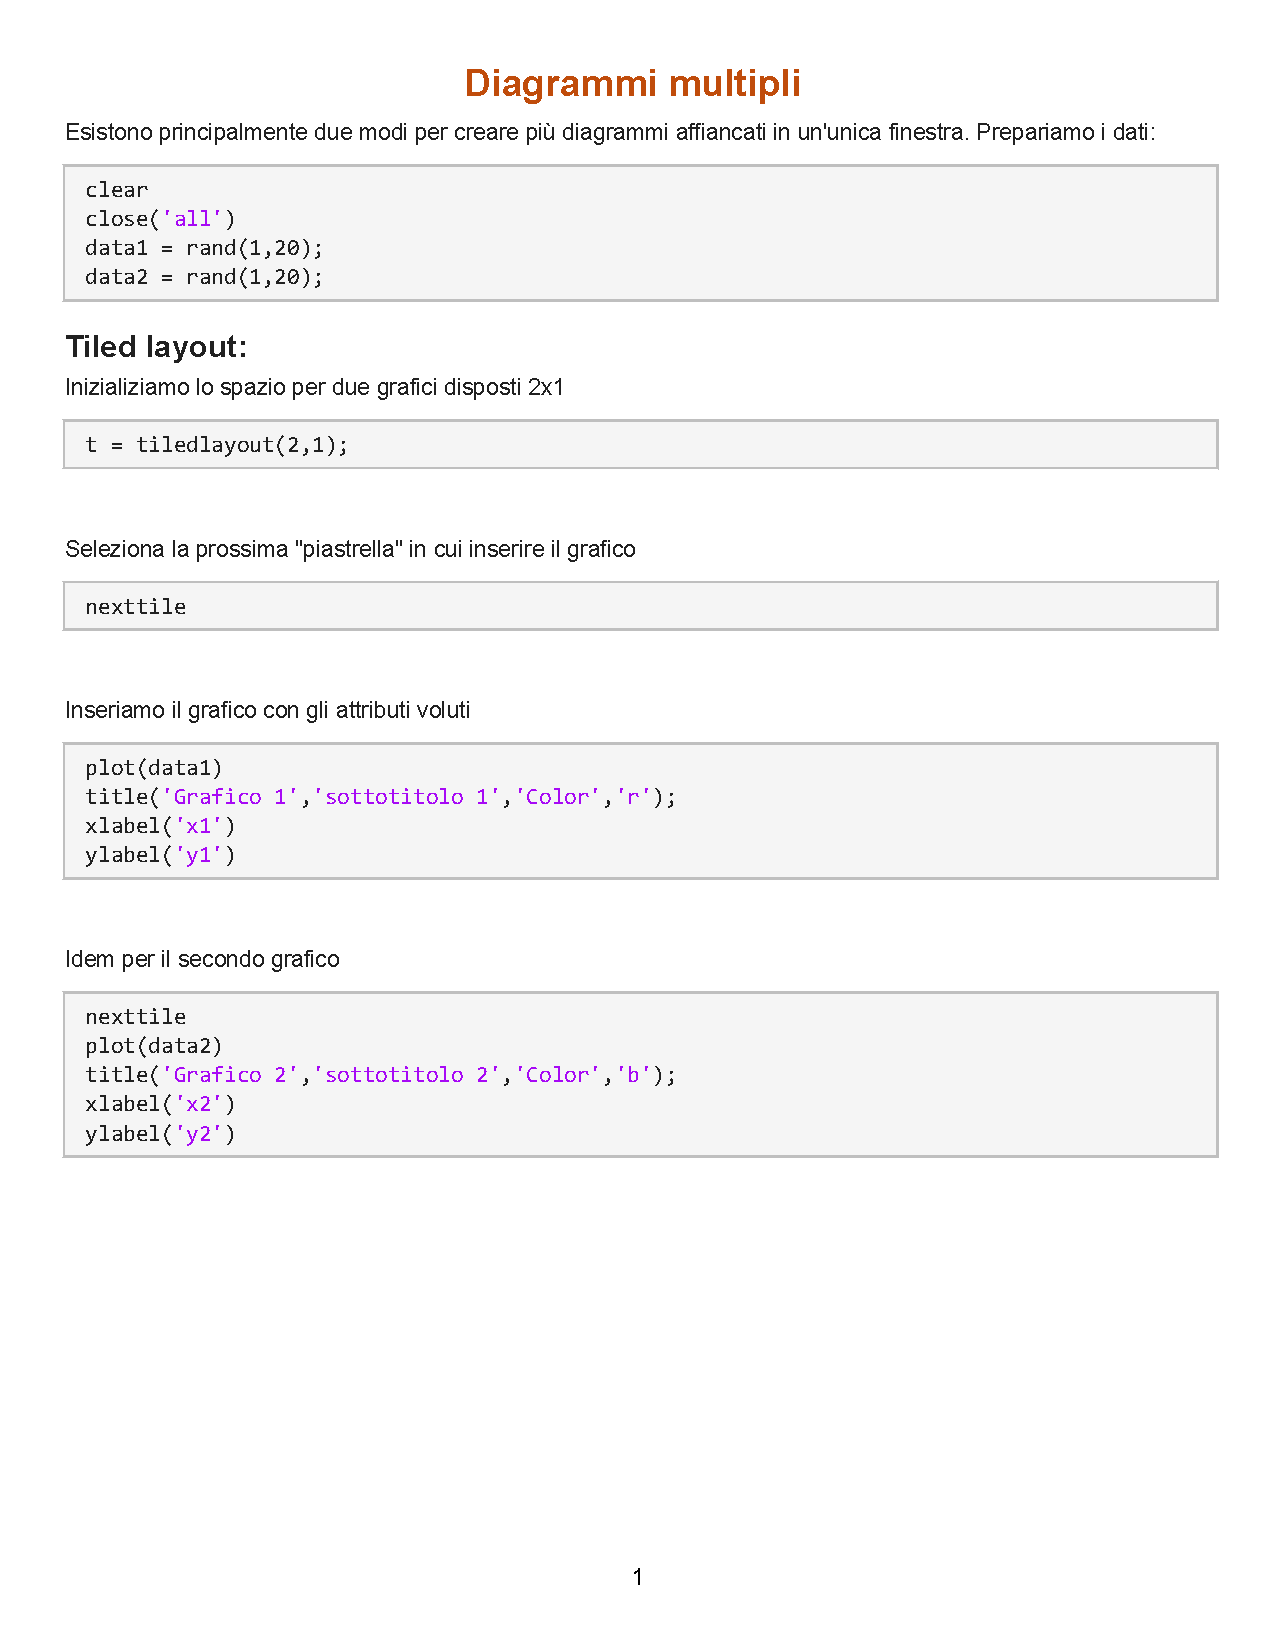
\includepdf[pages=-]{cap/TeoGrafici/Gestione_Diagrammi5}
 % Teoria con esempi Matlab 

%\part{Esercizi}
\chapter[Esercizi Elementary MatLab]{Esercizi del Elementary Mechanics Using 
Matlab}

\section{Ex2.01 Seconds}\label{sec:seconds}
\subsection{Testo esercizio}
\begin{itemize}
    \item[a)] Scrivi una funzione che calcola il numero di secondi, $s$ dati il 
    numero di ore, secondo la formula $$s = 3600*h$$
    
    \item[b)] Utilizzare uno script per trovare il numero di secondi in $1.5$, 
    $12$ e $24$ ore.
\end{itemize}

\subsection{Svolgimento}
L'esercizio è stato molto semplice e privo di difficoltà.

\subsection{Risultati}
\subsubsection{Testuali} 
\color{gray}\begin{verbatim}
In  1.5 ore ci sono  5400 secondi
In 12.0 ore ci sono 43200 secondi
In 24.0 ore ci sono 86400 secondi
\end{verbatim}
\color{black}

\subsubsection{Tabella}    
\providecommand*{\thead}[1]{\multicolumn{1}{c}{\bfseries #1}}%
\providecommand*{\unitHead}[1]{\multicolumn{1}{c}{(\si{#1})}}%

\begin{table}[h]%
\centering%
\begin{tabular}{S[table-format=-1.3]S[table-format=-1.3]}%
\toprule%
\thead{hours}&\thead{seconds}\\
\toprule%
1.50	&	5400.00 \\%
12.00	&	43200.00 \\%
24.00	&	86400.00 \\%
\bottomrule%
\end{tabular}%
\caption{table201}%
\label{tab:table201}%
\end{table}%
\newpage

\subsection{Codici usati}
\lstinputlisting[caption = {\nameref{fnc:hoursToSecond}},
linerange = {36-40}]
{cap/Elementary/src/function/hoursToSeconds.m}%

\lstinputlisting[title = {\nameref{scr:script201}},
linerange = {31-37}]
{cap/Elementary/src/script/script201.m}
 % 2.01 Seconds
\section{Ex2.02 Mass sphere}\label{sec:Mass_sphere}

\subsection{Testo esercizio}
\begin{itemize}
    \item[a)] Scrivi una funzione che calcoli la massa di una sfera 
    dato il suo raggio, $r$, e la densità di massa, $\rho$, secondo la 
    formula $$m=\rho\frac{4}{3}\pi r^3$$
    
    \item[b)] Usa uno script per trovare la massa di una sfera di 
    acciaio ($\rho=7500\frac{Kg}{m^3}$) di raggio $1mm$, $1m$ e $10m$.
\end{itemize}

\subsection{Svolgimento}
L'esercizio \'e stato semplice. Inizialmente avevo inserito $\rho=7500$ 
direttamente dentro la funzione, successivamente ho reputato opportuno 
inserire il dato via argomenti per rendere la funzione utile per 
qualsiasi tipo di sfera.

\subsection{Risultati}
\subsubsection{Testuali}
\color{gray}
\begin{verbatim}
>> scriptMassa
Una sfera d'acciaio di raggio 1.00e-03 m ha massa di 3.14e-05 Kg
Una sfera d'acciaio di raggio 1.00e+00 m ha massa di 3.14e+04 Kg
Una sfera d'acciaio di raggio 1.00e+01 m ha massa di 3.14e+07 Kg
>> 
\end{verbatim}
\color{black} 

\subsubsection{Tabella}    
\providecommand*{\thead}[1]{\multicolumn{1}{c}{\bfseries #1}}%
\providecommand*{\unitHead}[1]{\multicolumn{1}{c}{(\si{#1})}}%

\begin{table}[h]%
\centering%
\begin{tabular}{S[table-format=-1.3]S[table-format=-1.3]}%
\toprule%
\thead{radius}&\thead{mass}\\
\toprule%
0.00	&	0.00 \\%
1.00	&	31415.93 \\%
10.00	&	31415926.54 \\%
\bottomrule%
\end{tabular}%
\caption{table202}%
\label{tab:table202}%
\end{table}%
\newpage

\subsection{Codici usati}
\lstinputlisting[caption = {\nameref{fnc:massSphere}},
linerange = {48-52}]
{cap/Elementary/src/function/massSphere.m}

\lstinputlisting[title = {\nameref{scr:script202}},
linerange = {33-41}]
{cap/Elementary/src/script/script202.m} % 2.02 Spherical Mass
\section{Ex2.03 Angle}\label{sec:Angle}

\subsection{Testo esercizio}
\begin{itemize}
    \item[a)]Scrivere una funzione che dato un punto $(x, y)$ restituisca 
    l'angolo $\theta$ dall'asse $x$ usando la formula
    $$\theta = arctan\frac{y}{x}$$
    
    \item[b)]Trova gli angoli $\theta$ per i punti
    $$(1,1)\;(-1,1)\;(-1,-1)\;(1,-1)$$
    
    \item[c)] Come cambieresti la funzione per restituire valori di $\theta$ 
    nell'intervallo $[0, 2\pi]$?
\end{itemize}

\subsection{Svolgimento}
L'esercizio è stato di complessità media. I primi due punti sono stati 
semplici, applicando la funzione data. Per il punto \textit{c)} dopo 
un'accurata ricerca, ho scelto di utilizzare la funzione \verb|mod()| con 
l'accortezza in caso di:
\begin{description}
    \item[$mod=0 \& radianti > 0$] di riportare il risultato a $2\pi$
    
    \item[$mod=0 \& radianti < 0$] di mantenere il risultato a $0$
\end{description}

\subsection{Risultati}
\subsubsection{Testuali}
\color{gray}
\begin{verbatim}
>> script203
Il punto ( 1,  1) ha l'angolo di:  0.7854°,  0.0137 rad,  0.0137 rad in [0,2pi]
Il punto (-1,  1) ha l'angolo di: -0.7854°, -0.0137 rad,  6.2695 rad in [0,2pi]
Il punto (-1, -1) ha l'angolo di:  0.7854°,  0.0137 rad,  0.0137 rad in [0,2pi]
Il punto ( 1, -1) ha l'angolo di: -0.7854°, -0.0137 rad,  6.2695 rad in [0,2pi]
>> 
\end{verbatim}
\color{black}

\subsubsection{Tabella}    
\providecommand*{\thead}[1]{\multicolumn{1}{c}{\bfseries #1}}%
\providecommand*{\unitHead}[1]{\multicolumn{1}{c}{(\si{#1})}}%

\begin{table}[h]%
\centering%
\begin{tabular}{ccS[table-format=-1.3]S[table-format=-1.3]}%
\toprule%
\thead{Var1}&\thead{Var2}&\thead{rad}&\thead{wrap2pi}\\
\toprule%
( +1.00, +1.00)	&   45 &  0.79 & 0.79 \\%
( -1.00, +1.00)	&  135 &  2.36 & 2.36 \\%
( -1.00, -1.00)	& -135 & -2.36 & 3.93 \\%
( +1.00, -1.00)	&  -45 & -0.79 & 5.50 \\%
\bottomrule%
\end{tabular}%
\caption{table203}%
\label{tab:table203}%
\end{table}%
\pagebreak

\subsection{Codice usati}
\lstinputlisting[title = {\nameref{fnc:pointToAngle}},
linerange={47-52}]
{cap/Elementary/src/function/pointToAngle.m}

\lstinputlisting[title = {\nameref{scr:script203}},
linerange={31-45}]
{cap/Elementary/src/script/script203.m}

\lstinputlisting[title = {\nameref{fnc:radMap2Pi}},
linerange={33-41}]
{cap/Elementary/src/function/radMap2Pi.m} % 2.03 Angle
\section{Ex2.04 Unit vector}\label{sec:Unit_vector}

\subsection{Testo esercizio}
\begin{itemize}
    \item[a)] Scrivere una funzione che restituisce il vettore unitario 
    bidimensionale, $(u_x , u_y)$, corrispondente a un angolo $\theta$ con 
    l'asse $x$. Puoi usare la formula, $$(u_x , u_y)=(\cos\theta,\sin\theta)$$ 
    dove $\theta$ e' dato in radianti.
    
    \item[b)] Trova gli angoli $\theta$ per i vettori 
    $$0,\frac{\pi}{6},\frac{\pi}{3},\frac{\pi}{2},\frac{3\pi}{2}$$     
    
    \item[3)] Riscrivi la formula per avere l'argomento in gradi.
\end{itemize}

\subsection{Svolgimento}
La difficoltà dell'esercizio è stata quella di trovare delle funzioni e formule 
che andassero bene per i vari tipi di input \verb|radianti/gradi|. Dopo una 
piccola ricerca, ho trovato le funzioni \MATLAB \verb|sin(x), cos(x)| e 
\verb|sind(x), cosd(x)| per \verb|x| rispettivamente \verb|radianti| e 
\verb|gradi|.

\subsection{Risultato}
\color{gray}
\begin{verbatim}
L'angolo di +00 rad ha coordinate (+1.00, +0.00)
L'angolo di +00 gra ha coordinate (+1.00, +0.00)

L'angolo di +5.24e-01 rad ha coordinate (+0.87, +0.50)
L'angolo di +3.00e+01 gra ha coordinate (+0.87, +0.50)

L'angolo di +1.05e+00 rad ha coordinate (+0.50, +0.87)
L'angolo di +6.00e+01 gra ha coordinate (+0.50, +0.87)

L'angolo di +1.57e+00 rad ha coordinate (+0.00, +1.00)
L'angolo di +90 gra ha coordinate (+0.00, +1.00)

L'angolo di +4.71e+00 rad ha coordinate (-0.00, -1.00)
L'angolo di +270 gra ha coordinate (+0.00, -1.00)
\end{verbatim}
\color{black}
\subsubsection{Tabella}    
\providecommand*{\thead}[1]{\multicolumn{1}{c}{\bfseries #1}}%
\providecommand*{\unitHead}[1]{\multicolumn{1}{c}{(\si{#1})}}%

\begin{table}[h]%
\centering%
\begin{tabular}{S[table-format=-1.3]S[table-format=-1.3]c}%
\toprule%
\thead{Radianti}&\thead{Gradi}&\thead{Coordinate}\\
\toprule%
0.00	&	0.00	&	( +1.00, +0.00) \\%
0.52	&	30.00	&	( +0.87, +0.50) \\%
1.05	&	60.00	&	( +0.50, +0.87) \\%
1.57	&	90.00	&	( +0.00, +1.00) \\%
4.71	&	270.00	&	( -0.00, -1.00) \\%
\bottomrule%
\end{tabular}%
\caption{table204}%
\label{tab:table204}%
\end{table}%
\newpage

\subsection{Codice esercizio}
\lstinputlisting[caption = {Funzione unitVectorR},
linerange={40-45}]%
{cap/Elementary/src/function/unitVectorR.m}

\lstinputlisting[title = {Script Ex2.04},
linerange={3-17}]%
{cap/Elementary/src/script/script204.m}

\lstinputlisting[caption = {Funzione unitVectorD},
linerange={38-43}]%
{cap/Elementary/src/function/unitVectorD.m}
 % 2.04 Unit Vector
%\section{Ex2.05 Plotting Normal Distribution}\label{sec:NormalDistribution}

\subsection{Testo esercizio}
La funzione $f(x;\mu;\sigma)$ nota come distribuzione normale o gaussiana è 
data come 
$$f(x,\mu,\sigma) = \frac{1}{{\sigma\sqrt{2\pi}}}
e^{{{-\left({x-\mu}\right)^2}/{2\sigma^2}}}$$    
dove $\mu$ è la media e $\sigma$ è la deviazione standard.

\begin{itemize}
    \item[a)] Creare una funzione $normalDistribuition(x,mu,sigma)$ che 
    restituisce il valore di $f(x,\mu,\sigma)$.
    
    \item[b)] Usa questa funzione per tracciare la gaussiana per $-5<x<5$ con 
    $\mu=0$ e $\sigma=1$.
    
    \item[c)] Usa questa funzione per tracciare le gaussiane per $-5<x<5$ con 
    $\mu=0$ e $\sigma=2$ e $0.5$ nelle stesso diagramma.
    
    \item[d)] Usa questa funzione per tracciare le gaussiane per $-5<x<5$ con 
    $\sigma=1$ e $\mu=0$, $1$, $2$ in 3 diagrammi nelle stessa figura.
\end{itemize}
\subsection{Svolgimento}
L'esercizio \'e stato semplice. Inizialmente avevo inserito $\rho=7500$ 
direttamente dentro la funzione, successivamente ho reputato opportuno inserire 
il dato via argomenti per rendere la funzione utile per qualsiasi tipo di sfera.

\subsection{Codice esercizio}
\lstinputlisting[caption = {\nameref{fnc:NormalDistribution}},
linerange = {33-40}]
{cap/Elementary/src/function/normalDistribuition.m}
\pagebreak

\subsection{Grafici con codici}
\lstinputlisting[title = {Script Ex2.05-b},
linerange = {3-10}]
{cap/Elementary/src/script/script205b.m}
\begin{figure}[h]
    \centering
    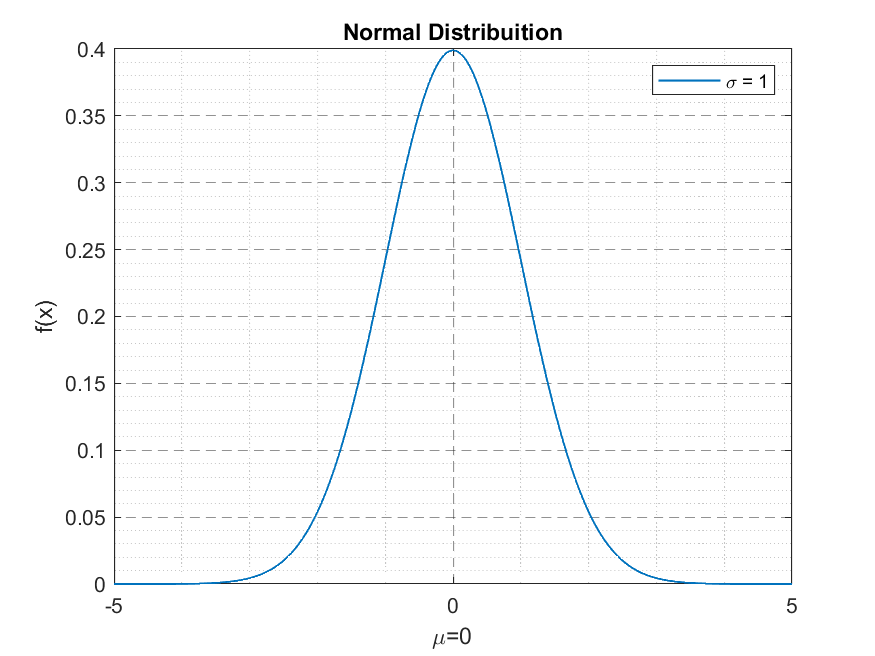
\includegraphics{cap/Elementary/img/script205b}
    \label{fig:script205b}
\end{figure}
\pagebreak

\lstinputlisting[title = {Script Ex2.05-c},
linerange = {33-40}]
{cap/Elementary/src/script/script205c.m}
\begin{figure}[h]
    \centering
    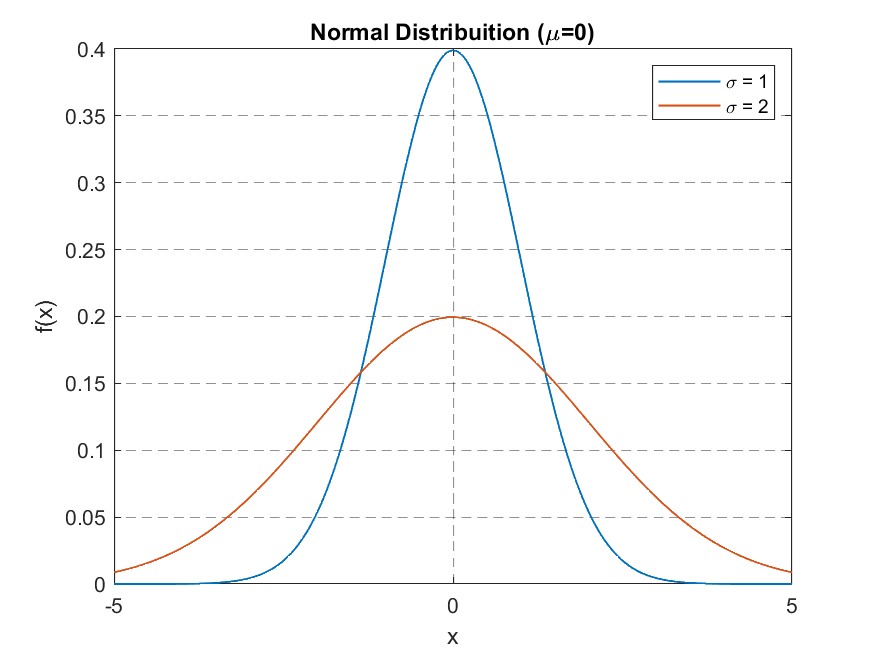
\includegraphics{cap/Elementary/img/script205c}
    \label{fig:plotscript205c}
\end{figure}
\pagebreak

\lstinputlisting[title = {Script Ex2.05-d},%
linerange ={3-17}]
{cap/Elementary/src/script/script205d.m}
\begin{figure}[h]
    \centering
    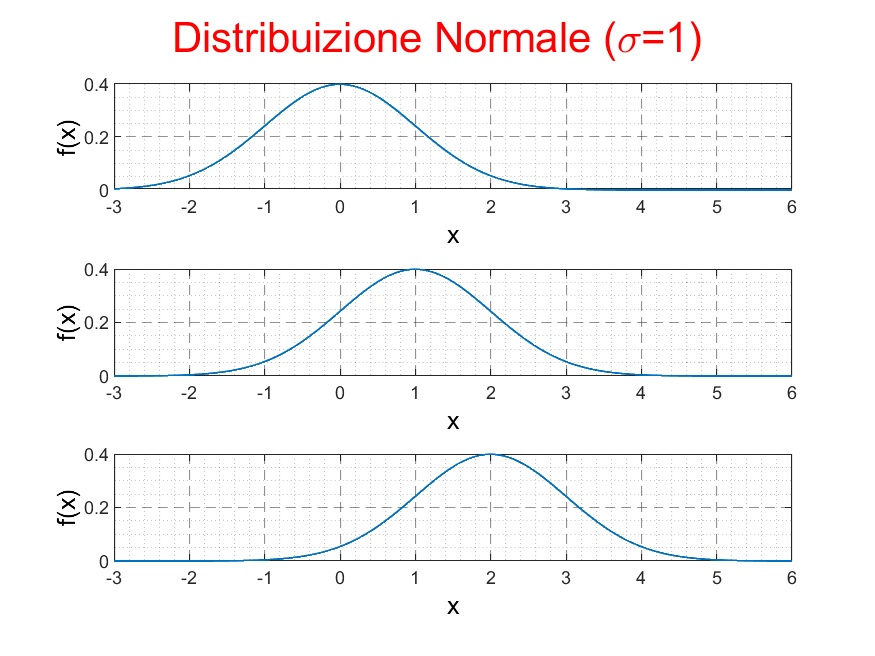
\includegraphics{cap/Elementary/img/script205d}
    \label{fig:plotscript205d}
\end{figure} % 2.05 Plotting Normal Distribution
%\section{Ex2.06 Plotting $1/x^n$}\label{1/x^n}
\subsection{Testo esercizio}
La funzione $f(x;n)$ è data come $f(x;n) =\frac{1}{x^{n}}$

\begin{itemize}
    \item[a)] Creare una funzione $fvalue(x,n)$ che restituisce il valore di $f(x,n)$.
        
    \item[b)] Usa questa funzione per tracciare $$f_1=\dfrac{1}{x},\quad 
    f_2=\dfrac{1}{x^2}, \quad f_3=\dfrac{1}{x^3}$$ nello stesso grafico per $-1<x<1$.
\end{itemize}

\subsection{Svolgimento}
L'esercizio è stato di base semplice. E' Bastato attenzionare \verb*|./| e \verb*|.^| per 
operare singolarmente su ogni elemento di matrici come se fosse un elemento a se stante e 
il resto è stato semplice.

\subsection{Risultato}
\begin{figure}[h]
    \centering
    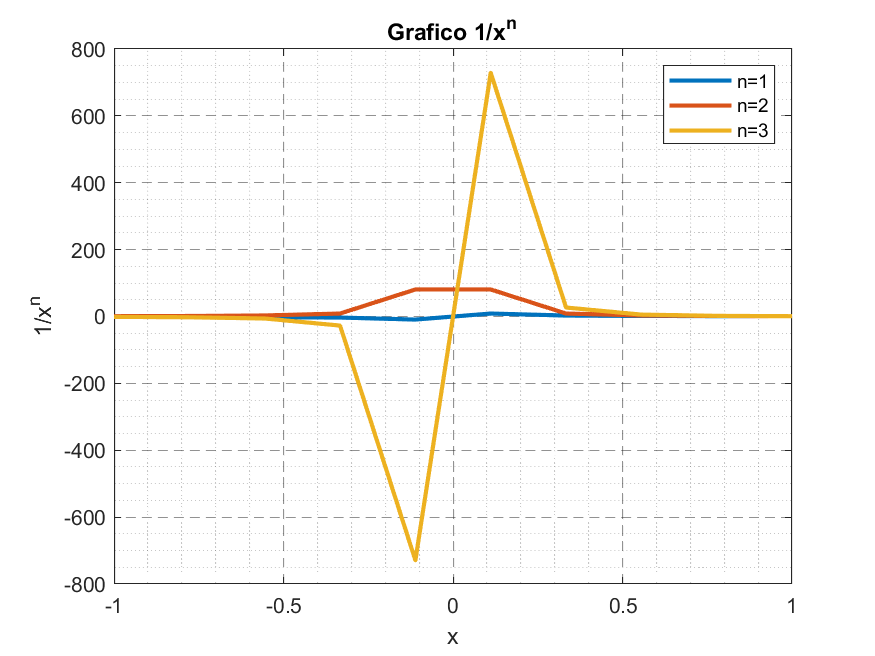
\includegraphics{cap/Elementary/img/script206}
    \GraphCap{$1/x^n$}
    \label{fig:script206}
\end{figure}
\newpage

\subsection{Codice esercizio}
\lstinputlisting[caption = {\nameref{fnc:fvalue}},
linerange={42-50}]
{cap/Elementary/src/function/fvalue.m}

\lstinputlisting[title = {Script Ex2.06}]
{cap/Elementary/src/script/script206.m}
 % 2.06 Plotting 1/x^n
%\section{Ex2.07 Plotting $\sin(x)/x^n$}\label{sec:Plotting_sin}

\subsection{Testo esercizio}
La funzione $g(x;n)$ è data come 
$$g(x;n) = \dfrac{\sin(x)}{x^n}$$

\begin{itemize}
    \item[a)] Creare una funzione $gvalue(x;n)$ che restituisce il valore di $g(x;n)$.
    
    \item[b)] Usa questa funzione per tracciare $$g_1=\dfrac{\sin(x)}{x},\quad 
    g_2=\dfrac{\sin(x)}{x^2}, \quad g_3=\dfrac{\sin(x)}{x^3}$$ nello stesso 
    grafico per $-5<x<5$.
\end{itemize}

\subsection{Svolgimento}
L'esercizio \'e stato semplice. Inizialmente avevo inserito $\rho=7500$ direttamente 
dentro la funzione, successivamente ho reputato opportuno inserire il dato via argomenti 
per rendere la funzione utile per qualsiasi tipo di sfera.

\subsection{Risultato}
\begin{figure}[h]
    \centering
    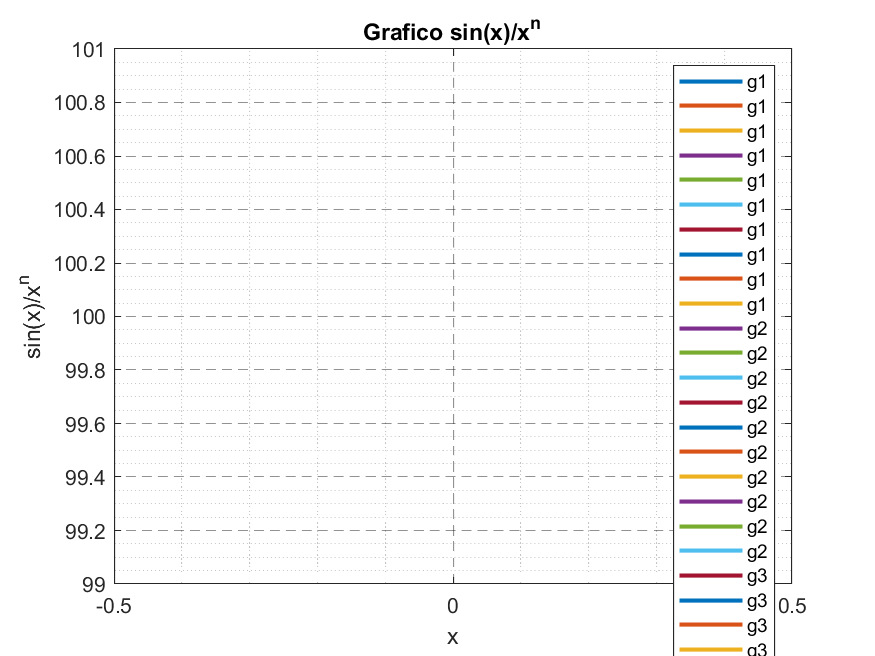
\includegraphics{cap/Elementary/img/script207}
    \GraphCap{$\sin(x)/x^n$}
    \label{fig:script207}
\end{figure}

\subsection{Codice esercizio}
\lstinputlisting[caption = {\nameref{fnc:gvalue}},
linerange={1-3}]
{cap/Elementary/src/function/gvalue.m}

\lstinputlisting[title = {Script Ex2.07}
,linerange={3-22}]
{cap/Elementary/src/script/script207.m} % 2.07 Plotting sin(x)/x^n
%\section{Ex2.08 Logistic map}\label{sec:LogisticMap}

\subsection{Testo esercizio}
La mappatura iterativa $$x(i+1)=rx(i)(1-x(i))$$ è chiamata \textbf{Logistic map}.

\begin{itemize}
    \item[a)] Scrivere una funzione $logisticMap(x,r)$ che ritorna il valore $x(i+1)$ 
    dati in input $x(i)$ ed $r$
    
    \item[b)] Scriver uno script con un loop per calcolare i primi $100$ passi della 
    mappa logistica partendo da $x(1)=0.5$. Memorizzare tutti i valori in una matrice $x$ 
    con $n=100$ elementi e traccia $x$ in funzione del numero di passaggi $i$.
    
    \item[c)] Esplora la mappa logistica per $$r_1=1.0\quad r_2=2.0\quad r_3=3.0\quad  
    r_4=4.0$$
    
\end{itemize}

\subsection{Svolgimento}
L'esercizio \'e stato semplice. Inizialmente avevo inserito $\rho=7500$ direttamente 
dentro la funzione, successivamente ho reputato opportuno inserire il dato via argomenti 
per rendere la funzione utile per qualsiasi tipo di sfera.

\subsection{Risultato}
\begin{figure}[h]
    \centering
    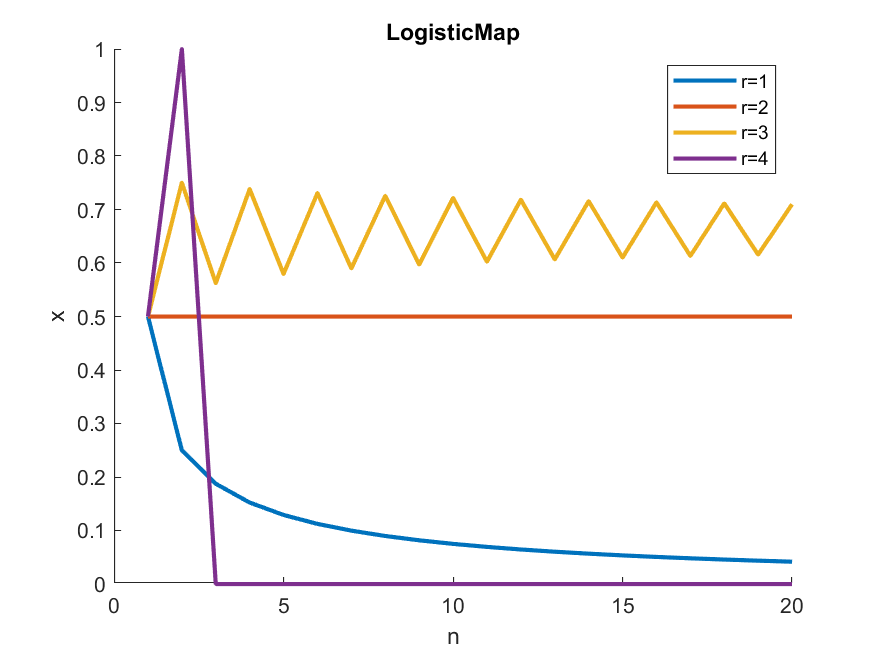
\includegraphics{cap/Elementary/img/script208}
    \GraphCap{$1/x^n$}
    \label{fig:script208}
\end{figure}

\subsection{Codice esercizio}
\lstinputlisting[caption = {\nameref{fnc:LogisticMap}},
linerange={1-3}]
{cap/Elementary/src/function/LogisticMap.m}

\lstinputlisting[title = {Script Ex2.08}]
{cap/Elementary/src/script/script208.m}
 % 2.08 Logistic Map
%\section{Ex2.09 Metodo di Eulero}\label{sec:Eulers_method}

\subsection{Testo esercizio}
Spesso si usa il metodo di \textbf{Eulero} per determinare il moto di un oggetto dato 
come l'accelerazione dipende dalla velocità e dalla posizione di un oggetto. 
$$\alpha(x,v) = \mathit{-kx-Cv}$$
Se conosciamo la posizione $\mathit{x}$ e la velocità $\mathit{v}$ in un tempo 
$\mathit{t(0)=0;\;\; x(0)=0\;\; e \;\;v(0)=1}$, possiamo usare il metodo di 
\textbf{Eulero} per trovare la posizione e la velocità dopo un piccolo $\Delta t:$

\begin{displaymath}
\begin{split}
&\mathit{v_1 = v(t_0 + \Delta t) = v(t_0) + \alpha(v(t_0),x(t_0))\Delta t} \\
&\mathrm{x_1 = v(t_0 + \Delta t) = x(t_0) + v(t_0)\Delta t} \\
&\mathsf{v_2 = v(t_1 + \Delta t) = v(t_1) + \alpha(v(t_1),x(t_1))\Delta t} \\
&\mathnormal{x_2 = v(t_1 + \Delta t) = x(t_1) + v(t_1)\Delta t} \\
\end{split}
\end{displaymath}
e cosi via.

\begin{itemize}
    \item[a)] Scrivere una funzione $\mathit{acceleration(x,v,k,C)}$ che restituisce 
    il valore di $\alpha(x,v) = -kx-Cv$.
    
    \item[b)] Scrivi uno script che calcoli i primi $100$ valori di $x(t_i)$ e $v(t_i)$ 
    quando $k=10$, $C=5$ e $\Delta t=0.01$. Traccia $x(t)$, $v(t)$ e $\alpha(t)$ in 
    funzione del tempo.
    
    \item[c)] Modifica la funzione per trovare $x(1)$ e $v(I)$ con    
    $\alpha(x,v)=k\sin(x)-Cv$.    
\end{itemize}

\subsection{Svolgimento}
L'esercizio è stato semplice. Il problema dell'esercizio, ovviamente era la corretta 
scrittura delle formule. Dopo un po' di ragionamento sono arrivata a scriverle 
correttamente. Per il \textit{punto C}, osservata bene la formula ho notato che 
differisce dala precedente solo per $-\sin(x)$ al posto di $x$, per cui ho semplicemente 
richiamato la prima con il $-\sin(x)$ al posto di $x$.

\subsection{Risultati}
\subsubsection{Grafico}
\begin{figure}[h]
    \centering
    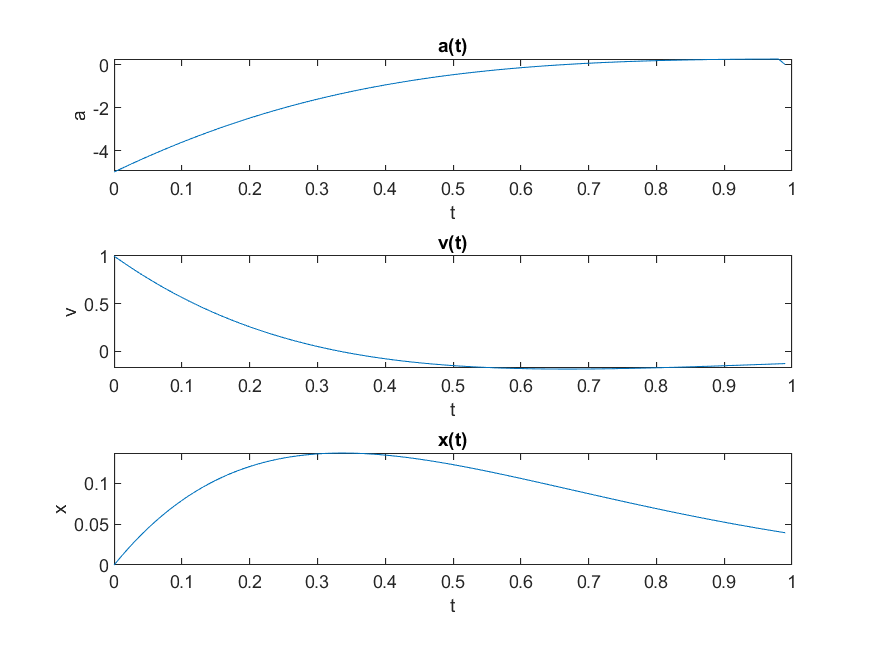
\includegraphics[width=0.7\linewidth]{cap/Elementary/img/script209}
    \GraphCap{$1/x^n$}
    \label{fig:script209}
\end{figure}
\pagebreak
\subsection{Codice esercizio}
\lstinputlisting[caption = {\nameref{fnc:acceleration}},
linerange={1-3}]
{cap/Elementary/src/function/acceleration.m}

\lstinputlisting[title = {script209},
linerange={3-35}]
{cap/Elementary/src/script/script209.m}

\lstinputlisting[title = {\nameref{fnc:acceleration2}},
linerange={1-3}]
{cap/Elementary/src/function/acceleration2.m}

\subsection{CHANGELOG Ex2.09}
\begin{changelog}[author=Cristina, simple, title={Modifiche alla funzione},%
    label=chgf:Eulers_method, sectioncmd=\subsubsection*]
    
    \shortversion{v=3.0.1, date=2020-09-13,%
        changes={Cambiati l'ordine degli argomenti e aggiornata la 
            validazione degli stessi}}      
    
    \shortversion{v=3.0.0, date=2020-09-13,%
        changes={Impostata la variabile \textit{rho} come argomento di 
            input}}
    
    \shortversion{v=2.0.0, date=2020-09-10, changes=Inserita la validazione 
    dell'output}   
    \shortversion{v=1.0.0, date=2020-09-03, changes=Commenti}
    \shortversion{v=0.1.0, date=2020-09-03, changes=Initial beta}
\end{changelog}

\begin{changelog}[author=Cristina, simple, title={Modifiche allo script},% 
    label=chg:script209, sectioncmd=\subsubsection*]
    
    \shortversion{v=1.0.0, date=2020-09-03, changes=Commenti}
    \shortversion{v=0.1.0, date=2020-09-03, changes=Initial beta}
\end{changelog} % 2.09 Eulero
%\section{Ex2.10 Throwing two dice}\label{sec:Throwing_two_dice}

\subsection{Testo esercizio}
Lanciare una coppia di dadi a sei facce e sommarne il numero di ciascuno dei dadi: 
$$Z=X1+X2$$ dove $Z$ è la somma dei risultati dei dadi 1, $X1$, e 2, $X2$. Eseguire 
questo esperimento molte volte $(N)$, e trovarne la \textit{media} e la 
\textit{deviazione standard}.
La media,$\langle Z\rangle$ è stimata da:
$$\langle Z\rangle=\frac{1}{N}\sum_{j=1}^{N}Z_j $$ 

la deviazione standard, $\Delta Z$, invece:
$$\Delta Z=\frac{1}{N-1}\sum_{j=1}^{N}\left(Z_j-Z\right)^2 $$

\begin{itemize}
    \item[a)] Scrivere una funzione che restituisce una matrice di $N$ valori per $Z$.
    
    \item[b)] Scrivere una funzione che restituisce una stima della media di una matrice 
    $Z$ utilizzando la formula fornita.

    \item[c)] Scrivere una funzione che restituisce una stima della deviazione standard 
    di una matrice $Z$ utilizzando la formula fornita.
    
    \item[d)] Trova la media e la deviazione standard per $N=100$ lanci di due dadi.
\end{itemize}

\subsection{Svolgimento}
L'esercizio è stato molto divertente. Alcuni problemi sono sorti per colpa di 
un errore di stampa nella formula, che \verb*|google.it| ha prontamente 
risolto. Questo esercizio mi ha anche permesso di creare tabelle con 
associazione di dati, tipo percentuale e conteggio di ogni singola somma 
($1-12$)
\pagebreak

\subsection{Risultati}
\subsubsection{Grafico}
\begin{figure}[h]
    \centering
    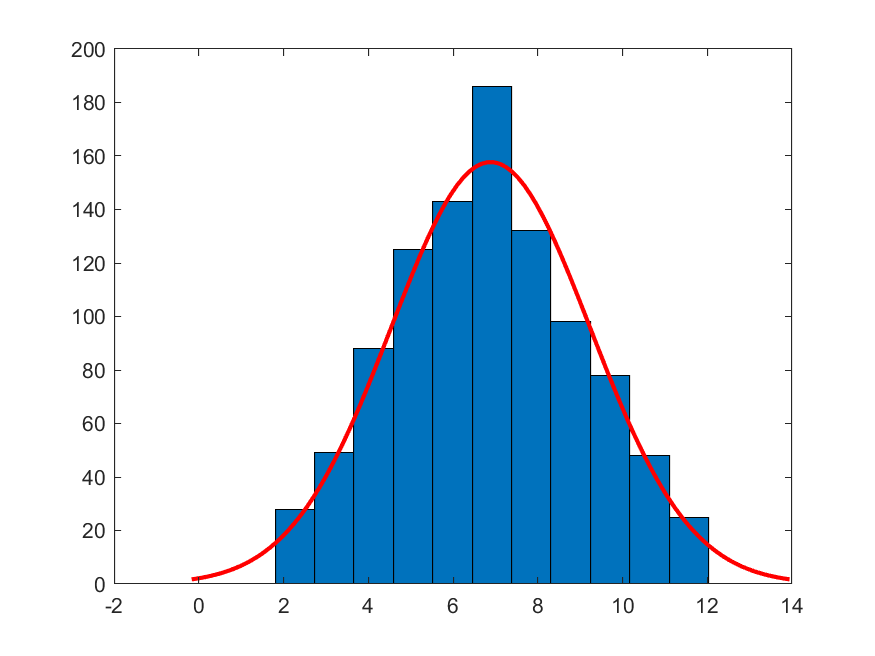
\includegraphics[width=0.7\linewidth]{cap/Elementary/img/script210}
    \GraphCap{Lancio dei dadi}
    \label{fig:script210}
\end{figure}
\subsubsection{Tabella}
\providecommand*{\thead}[1]{\multicolumn{1}{c}{\bfseries #1}}%
\providecommand*{\unitHead}[1]{\multicolumn{1}{c}{\si{#1}}}%

\begin{table}[h]%
\centering%
\begin{tabular}{S[table-format=-1.3]S[table-format=-1.3]S[table-format=-1.3]}%
\toprule%
\thead{throwDice}&\thead{GroupCount}&\thead{Percent}\\
\toprule%
2.00	&	28.00	&	2.80 \\%
3.00	&	49.00	&	4.90 \\%
4.00	&	88.00	&	8.80 \\%
5.00	&	125.00	&	12.50 \\%
6.00	&	143.00	&	14.30 \\%
7.00	&	186.00	&	18.60 \\%
8.00	&	132.00	&	13.20 \\%
9.00	&	98.00	&	9.80 \\%
10.00	&	78.00	&	7.80 \\%
11.00	&	48.00	&	4.80 \\%
12.00	&	25.00	&	2.50 \\%
\bottomrule%
\end{tabular}%
\caption{table210}%
\label{tab:table210}%
\end{table}%
\pagebreak

\subsection{Codice esercizio}
\lstinputlisting[caption = {Funzione ThrowingTwoDice},
linerange={32-42}]
{cap/Elementary/src/function/ThrowingTwoDice.m}

%\lstinputlisting[caption = {Funzione myMean}, label={lst:MyMean}]
%{cap/Elementary/src/function/myMean.m}

%\lstinputlisting[caption = {Funzione myStd}]
%{cap/Elementary/src/function/myStd.m}

\lstinputlisting[title = {Script Ex2.10},
linerange={3-16}]
{cap/Elementary/src/script/script210.m}
 % 2.10 Throwing two dice
%\section{Ex2.11 Reading data}\label{sec:Reading_data}

\subsection{Testo esercizio}
Il file \verb|trajectory.dat| contiene un elenco di numeri:\\   
\begin{tabular}{ccc}
    $t0$    & $x0$      & $y0$    \\
    $t1$    & $x1$      & $y1$    \\
    $\dots$ & $\dots$   & $\dots$ \\
    $tn$    & $xn$      & $yn$    \\
\end{tabular}\\
corrispondente al tempo $t(i)$ misurato in secondi e alle posizioni $x(i)$ e 
$y(i)$  misurato in metri per la traiettoria di un proiettile.
    
\begin{itemize}
    \item[a)] Leggere il file di dati, e popolare le matrici $t$, $x$ e $y$.
        
    \item[b)] Tracciare le posizioni $x$ e $y$ in funzione del tempo in due 
    grafici uno sopra l'altro.
        
    \item[c)] Tracciare le posizioni $(x, y)$ dell'oggetto in un grafico 
    con $x$ e $y$ sui due assi.
\end{itemize}

\subsection{Svolgimento}
Per questo esercizio ho deciso di usare le funzioni integrate dell'IDE di 
MATLAB che offrono una gestione dei file molto più comoda rispetto a quella con 
\verb*|fopen()|. Infatti con un file correttamente formato, basta una sola 
istruzione per importare i dati da un file. Poi con tre semplicissime 
assegnazioni, ottengo le tre variabili richieste. In seguito, ho deciso di 
mostrare tutti i 3 grafici insieme per rendere visibile in un'unica finestra 
tutti i risultati.
\subsection{Grafico}
\begin{figure}[h]
    \centering
    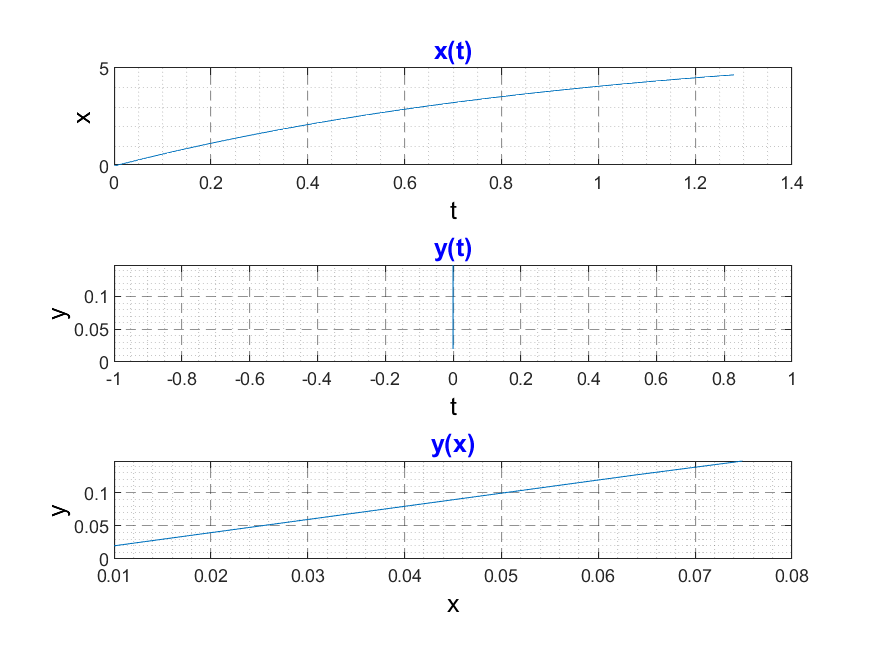
\includegraphics{cap/Elementary/img/script211}
    \label{fig:script211}
\end{figure}

\subsection{Codice esercizio}
\lstinputlisting[title = {\nameref{sec:script211}},
linerange={3-25}]
{cap/Elementary/src/script/script211.m} % 2.11 Reading data
%\section{Ex2.12 Data-set}\label{sec:Data_set}

\subsection{Testo esercizio}
Il file \textit{velocityy.dat} contiene un elenco di valori cosi disposti:\\

\begin{tabular}{cc}
    $t0$&$v0$\\
    $t1$&$v1$\\
    $..$&$..$\\
    $tn$&$vn$\\
\end{tabular}\\

corrispondenti al tempo $t(i)$, misurato in secondi, e alla velocità $v(i)$, 
misurata in metri al secondo, per la traiettoria di un proiettile.

\begin{itemize}
    \item[a)] Leggere il file di dati, e popolare le matrici $t$ e $v$.
    
    \item[b)] Graficare $v$ in funzione di $t$.
 
    \item[c)] Tracciare le posizioni $(x, y)$ dell'oggetto in un plot con $x$ e 
    $y$ sui due grafici, uno sopra l'altro.
\end{itemize}   

\subsection{Svolgimento}
L'esercizio \'e stato semplice. Inizialmente avevo inserito $\rho=7500$ 
direttamente dentro la funzione, successivamente ho reputato opportuno inserire 
il dato via argomenti per rendere la funzione utile per qualsiasi tipo di sfera.

\subsection{Codici esercizio}
\lstinputlisting[title = {\nameref{scr:script212}},
linerange={3-23}]
{cap/Elementary/src/script/script212.m}
\pagebreak

\subsection{Grafico}
\begin{figure}[h]
    \centering
    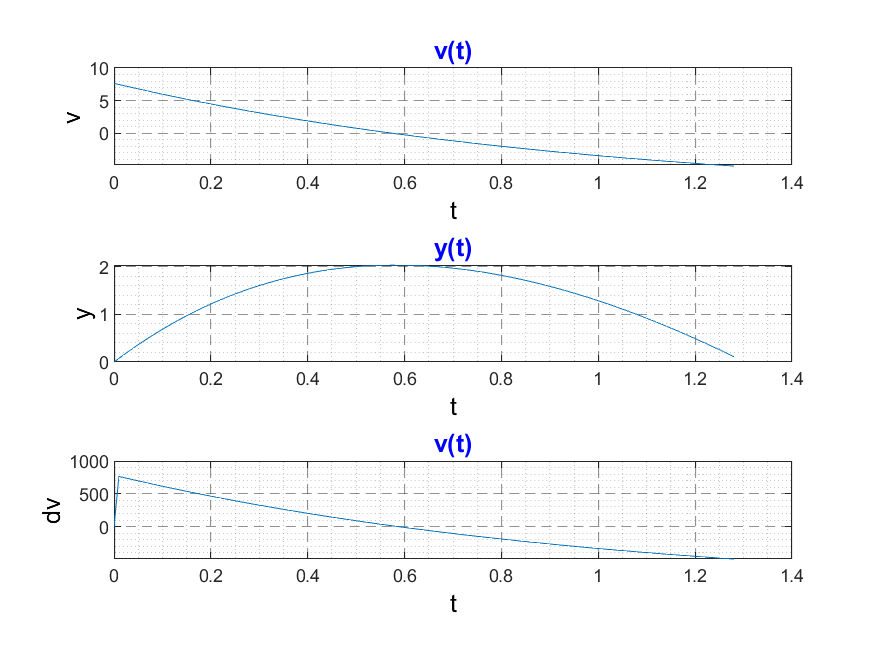
\includegraphics{cap/Elementary/img/script212}
    \GraphCap{Data-set}
    \label{fig:script212}
\end{figure}

 % 2.12 data-set % Esercizi dal cap2 

\part{Appendici}
\appendix
%\chapter{Funzioni di utilità negli script}

%\section{myGrid}\label{fnc:myGrid}

\subHeadMatlab{Sintassi}
\lstinputlisting[linerange = {31-31}, 
firstnumber=33,frameshape={RYRYNYYYY}{yny}{yny}{RYRYNYYYY}]
{cap/FuncUtility/src/myGrid.m}%

\subHeadMatlab{Argomenti}
\subsubsection{Input:}
\textit{none}

\subsubsection{Output:}
\textit{none}

\subHeadMatlab{Descrizione istruzioni}
La funzione serve ad impostare la grafica dei vari grafici. Creata solamente 
per evitare di riscrivere gli stessi comandi ogni volta, ed avere una grafica 
uguale per ogni grafico usato. 

\lstinputlisting[linerange = {32-37},firstnumber=32]
{cap/FuncUtility/src/myGrid.m}%

\subHeadMatlab{CHANGELOG}
\begin{changelog}[author=\CGC, simple, 
    title={Modifiche alla funzione}, 
    label=chgf:myGrid, sectioncmd=\subsubsection*]
        
    \shortversion{v=1.0.0, date=2020-09-03,
         changes={Inizializzazione funzione}}
\end{changelog}
\newpage
\subsubsection{Listato completo}
\lstinputlisting[title = myGrid, basicstyle=\scriptsize]
{cap/FuncUtility/src/myGrid.m}%      % Gestioner griglia
%\section{myLabelPlot}\label{fnc:myLabelPlot}

\subHeadMatlab{Sintassi}
\lstinputlisting[linerange = {33-33}, 
firstnumber=33,frameshape={RYRYNYYYY}{yny}{yny}{RYRYNYYYY}]
{cap/FuncUtility/src/myLabelPlot.m}%

\subHeadMatlab{Argomenti}
\subsubsection{Input:}
\lstinputlisting[linerange = {35-39}, firstnumber=36,basicstyle=\small]
{cap/FuncUtility/src/myLabelPlot.m}%

\begin{tcolorbox}
    
    \begin{description} 
\setlength{\itemindent}{-.2in}%%%%%% identa la lista
    \item[\textit{titlePlot:}] \verb|(1,1) string {mustBeNonempty}.|\\
    Scalare. Rappresenta il titolo del grafico. Deve essere una necessariamente 
    una stringa.
    
    \item[\textit{xAxe:}] \verb|(1,1) string = 'X'.|\\
    Scalare. Rappresenta l'etichetta da dare all'asse \textbf{X}. Deve essere 
    una necessariamente una stringa, se mancante si inserirà un valore di 
    default. Se non si vuole l'etichetta, basta inserire un valore vuoto.
    
    \item[\textit{xAxe:}] \verb|(1,1) string = 'Y'.|\\
    Scalare. Rappresenta l'etichetta da dare all'asse \textbf{X}. Deve essere 
    una necessariamente una stringa, se mancante si inserirà un valore di 
    default. Se non si vuole l'etichetta, basta inserire un valore vuoto.
\end{description}
\end{tcolorbox}

\subsubsection{Output:}
\textit{none}

\subHeadMatlab{Descrizione istruzioni}
\lstinputlisting[linerange = {41-44}, firstnumber=41, basicstyle=\small]
{cap/FuncUtility/src/myLabelPlot.m}%

\subHeadMatlab{CHANGELOG}
\begin{changelog}[author=\CGC, simple, title={Modifiche alla funzione}, 
    label=chgf:myLabelPlot, sectioncmd=\subsubsection*]
    
    \shortversion{v=1.0.0, date=2020-09-03,
         changes={Inizializzazione funzione}}
\end{changelog}
\newpage
\subsubsection{Listato completo}
\lstinputlisting[title = myLabelPlot, basicstyle=\scriptsize]
{cap/FuncUtility/src/myLabelPlot.m}% % Gestione plot
%\section{Moto browniano}

\subsection{Testo esercizio}
Creare un programma che simuli un moto browniano con queste caratteristiche.
\begin{itemize}

    \item Richieda \textit{\textbf{n}} misure random comprese tra 0 e 1
    \item setti una variabile opportuna che
    \begin{itemize}
        \item Aumenti di 1 se il valore della misura è minore di 0.5
        \item Diminuisca di 1 in caso contrario.
    \end{itemize}
    \item Esegua più volte l'esperimento, salvando di volta in volta il risultato in un array.
    \item Inserisca in un istogramma i risultati delle varie prove.
    
\end{itemize}
\pagebreak
\subsection{Codice esercizio}
\lstinputlisting[caption = {Moto browniano}, style=Matlab-editor]
{cap/cap1/src/Moto_Browniano.m}

\subsection{Risultato}
\begin{figure}[h]
    \centering
    \includegraphics[width=0.8\linewidth]{cap/cap1/img/plot103.png}
    \caption{Moto browniano \textit{(nP=100 - nO=10000)}}
    \label{fig:plot103}
    
\end{figure}


 % 2.03 Angle
%\section{Ex2.04 Unit vector}\label{sec:Unit_vector}

\subsection{Testo esercizio}
\begin{itemize}
    \item[a)] Scrivere una funzione che restituisce il vettore unitario 
    bidimensionale, $(u_x , u_y)$, corrispondente a un angolo $\theta$ con 
    l'asse $x$. Puoi usare la formula, $$(u_x , u_y)=(\cos\theta,\sin\theta)$$ 
    dove $\theta$ e' dato in radianti.
    
    \item[b)] Trova gli angoli $\theta$ per i vettori 
    $$0,\frac{\pi}{6},\frac{\pi}{3},\frac{\pi}{2},\frac{3\pi}{2}$$     
    
    \item[3)] Riscrivi la formula per avere l'argomento in gradi.
\end{itemize}

\subsection{Svolgimento}
La difficoltà dell'esercizio è stata quella di trovare delle funzioni e formule 
che andassero bene per i vari tipi di input \verb|radianti/gradi|. Dopo una 
piccola ricerca, ho trovato le funzioni \MATLAB \verb|sin(x), cos(x)| e 
\verb|sind(x), cosd(x)| per \verb|x| rispettivamente \verb|radianti| e 
\verb|gradi|.

\subsection{Risultato}
\color{gray}
\begin{verbatim}
L'angolo di +00 rad ha coordinate (+1.00, +0.00)
L'angolo di +00 gra ha coordinate (+1.00, +0.00)

L'angolo di +5.24e-01 rad ha coordinate (+0.87, +0.50)
L'angolo di +3.00e+01 gra ha coordinate (+0.87, +0.50)

L'angolo di +1.05e+00 rad ha coordinate (+0.50, +0.87)
L'angolo di +6.00e+01 gra ha coordinate (+0.50, +0.87)

L'angolo di +1.57e+00 rad ha coordinate (+0.00, +1.00)
L'angolo di +90 gra ha coordinate (+0.00, +1.00)

L'angolo di +4.71e+00 rad ha coordinate (-0.00, -1.00)
L'angolo di +270 gra ha coordinate (+0.00, -1.00)
\end{verbatim}
\color{black}
\subsubsection{Tabella}    
\providecommand*{\thead}[1]{\multicolumn{1}{c}{\bfseries #1}}%
\providecommand*{\unitHead}[1]{\multicolumn{1}{c}{(\si{#1})}}%

\begin{table}[h]%
\centering%
\begin{tabular}{S[table-format=-1.3]S[table-format=-1.3]c}%
\toprule%
\thead{Radianti}&\thead{Gradi}&\thead{Coordinate}\\
\toprule%
0.00	&	0.00	&	( +1.00, +0.00) \\%
0.52	&	30.00	&	( +0.87, +0.50) \\%
1.05	&	60.00	&	( +0.50, +0.87) \\%
1.57	&	90.00	&	( +0.00, +1.00) \\%
4.71	&	270.00	&	( -0.00, -1.00) \\%
\bottomrule%
\end{tabular}%
\caption{table204}%
\label{tab:table204}%
\end{table}%
\newpage

\subsection{Codice esercizio}
\lstinputlisting[caption = {Funzione unitVectorR},
linerange={40-45}]%
{cap/Elementary/src/function/unitVectorR.m}

\lstinputlisting[title = {Script Ex2.04},
linerange={3-17}]%
{cap/Elementary/src/script/script204.m}

\lstinputlisting[caption = {Funzione unitVectorD},
linerange={38-43}]%
{cap/Elementary/src/function/unitVectorD.m}
 % 2.04 Unit Vector
 % Funzioni commentate  
\chapter{Funzioni usate}

\section{hoursToSecond}\label{fnc:hoursToSecond}

\subHeadMatlab{Sintassi}
\lstinputlisting[linerange = {36-36},
basicstyle=\large, numbers=none]
{cap/Elementary/src/function/hoursToSeconds.m}%

\subHeadMatlab{Descrizione breve}
Calcola il numero di secondi contenute in un dato numero di ore.

\subHeadMatlab{Input}
\begin{tcolorbox}
    \begin{description} 
\setlength{\itemindent}{-.2in}
    \item[\textit{hours:}] \verb| double {mustBeNonNegative}.|\\
    Matrice. Ogni singolo elemento della matrice deve contenere un numero di 
    ore che verrà convertito in secondi autonomamente.
\end{description}
\end{tcolorbox}

\subHeadMatlab{Output}
\begin{tcolorbox}
\begin{description}
\setlength{\itemindent}{-.2in}
    \item[\textit{seconds:}] \verb|size(hours)| \\
     Matrice. Numero di secondi dati alla conversione delle ore. La dimensione 
     sarà la stessa di \verb|hours|
\end{description}
\end{tcolorbox}

\subHeadMatlab{Vedere anche}
{\color{gray} NONE}

\subHeadMatlab{Descrizione estesa}
La funzione è molto semplice, prende in ingresso un valore in ore 
e lo converte in secondi. La formula utilizzata nella conversione 
è semplicemente: 
$$s=h*3600$$
\lstinputlisting[linerange = {38-38}, firstnumber=46]
{cap/Elementary/src/function/hoursToSeconds.m}%
\pagebreak

\subHeadMatlab{CHANGELOG}
\begin{changelog}[author=\CGC, simple, title={Modifiche alla funzione}, 
    label=chgf:hoursToSecond, sectioncmd=\subsubsection*]
         
    \shortversion{v=1.0.1, date=20/09/2022,
         changes={Insertiti commenti}}
     
    \shortversion{v=1.0.0, date=20/09/2022,
         changes={Inizializzazione funzione}}
\end{changelog}
\newpage
%\subsubsection{Listato completo}
%\lstinputlisting[title = hoursToSeconds, basicstyle=\scriptsize]
%{cap/Elementary/src/function/hoursToSeconds.m}%
\section{massSphere}\label{fnc:massSphere}

\subHeadMatlab{Sintassi}
\lstinputlisting[linerange = {46-46}, basicstyle=\large,
numbers=none]
{cap/Elementary/src/function/massSphere.m}

\subHeadMatlab{Descrizione breve}
Calcola, dato un $\rho$ specifico del materiale, la massa di una 
sfera d'acciaio, dato il raggio.

%\subHeadMatlab{Argomenti}

\subHeadMatlab{Input}
\begin{tcolorbox}
\begin{description}
\setlength{\itemindent}{-.2in}
   
   \item[\textit{rho}] \verb|(1,1) {mustBePositive}|\\
    Scalare, necessariamente con elementi positivi. Ogni conversione può essere 
    riferita solo ad un tipo di materiale.
    
    \item[\textit{radius}] \verb|{mustBePositive} = 1|\\
    Matrice. Ogni singolo elemento di essa verrà considerato come un 
    raggio. Se non dovesse esserci default pari a 1 
    metro.
\end{description}
\end{tcolorbox}

\subHeadMatlab{Output}
\begin{tcolorbox}
    \begin{description}   
\setlength{\itemindent}{-.2in} 

        \item[\textit{mass}] \verb|size(radius)|\\
        Matrice i cui elementi corrispondono alle masse di sfere di raggio 
        corrispondenti agli elementi della matrice d'ingresso.
    \end{description}  
\end{tcolorbox}

\subHeadMatlab{Vedere anche}
{\color{gray} NONE}

\subHeadMatlab{Descrizione estesa}
La formula utilizzata é quella per il calcolo nella conversione 
ed é semplicemente: 
$$m=\rho\frac{4}{3}\pi r^3$$
\lstinputlisting[ linerange = {48-48}, firstnumber=48]
{cap/Elementary/src/function/massSphere.m}
\pagebreak


\subHeadMatlab{CHANGELOG}
\begin{changelog}[author=\CGC, simple, 
    title={Modifiche alla funzione}, 
    label=chgf:massSphere, sectioncmd=\subsubsection*]

    \shortversion{v=2.0.0, date=14/09/22, 
        changes=Inserita la variabile rho come argomento.}
       
    \shortversion{v=1.0.1, date=04/09/22, 
        changes=Insertiti commenti}
    
    \shortversion{v=1.0.0, date=03/09/22, 
        changes=Inizializzazione funzione}
\end{changelog}

%\subsubsection{Listato completo}
%\lstinputlisting[title = massSphere, basicstyle=\scriptsize]
%{cap/Elementary/src/function/massSphere.m}%
\section{pointToAngle}\label{fnc:pointToAngle}

\subHeadMatlab{Sintassi}
\lstinputlisting[ linerange = {47-47},
basicstyle=\large, numbers=none]
{cap/Elementary/src/function/pointToAngle.m}

\subHeadMatlab{Descrizione breve}
Dato un punto, o una serie di punti $P$, restituisce l'angolo che 
si forma tra la retta passante per $O(0,0)$ e il punto $P(x,y)$, 
e l'asse $x$.

\subHeadMatlab{Argomenti}

\subsubsection{Input:}
\begin{tcolorbox}
    \begin{description}
\setlength{\itemindent}{-.2in}
        
        \item[\textit{Axes:}] \verb|(:,2) double {mustBeNumeric}|\\
        Vettore a due colonne. In questo modo ogni conversione 
        può essere riferita solo ad un tipo di materiale
    \end{description}
\end{tcolorbox}

\subsubsection{Output}
\begin{tcolorbox}
    \begin{description}        
        \item[\textit{radiant:}] \verb|(length(Axes)) double.|\\
        Risultato del calcolo dell'angolo in radianti.
        
        \item[\textit{wrapZero2Pi:}] \verb|(length(Axes)) double.|\\
        Risultato del calcolo dell'angolo in radianti tra [0, 2*pi].
    \end{description}  
\end{tcolorbox}

\subHeadMatlab{Vedere anche}
{\nameref{fnc:radMap2Pi}}

\subHeadMatlab{Descrizione estesa}
Anche se l'$arcotangente$ restituisce un valore in radianti, ho pensato di far 
restituire alla funzione anche i gradi corrispondenti, usando le due formule:
$$ rad = \arctan\left( \frac{y}{x} \right) \qquad
   deg = \frac{\left( rad*180\right) }{\pi}$$

\lstinputlisting[ linerange = {49-50}, firstnumber=49]
{cap/Elementary/src/function/pointToAngle.m}
\pagebreak

\subHeadMatlab{CHANGELOG}
\begin{changelog}[author=\CGC, simple,
    title={Modifiche alla funzione}, 
    label=chg:pointToAngle, sectioncmd=\subsubsection*]
    
    \shortversion{v=2.0.0, date=2020-09-13, 
        changes=Inserita la validazione dell'output}
    
    \shortversion{v=1.0.1, date=2020-09-04, 
        changes=Insertiti commenti}
    
    \shortversion{v=1.0.0, date=2020-09-03, 
        changes=Inizializzazione funzione}
    
\end{changelog}
%\newpage
%\subsubsection{Listato completo}
%\lstinputlisting[title = pointToAngle, basicstyle=\scriptsize]
%{cap/Elementary/src/function/pointToAngle.m}
\section{radMap2Pi}\label{fnc:radMap2Pi}

\subHeadMatlab{Sintassi}
\lstinputlisting[ linerange = {34-34},
basicstyle=\large, numbers=none]
{cap/Elementary/src/function/radMap2Pi.m}

\subHeadMatlab{Descrizione breve}
Dato un angolo in radianti, lo mappa in un range di ${0, 2\pi}$ 

\subHeadMatlab{Argomenti}
\subsubsection{Input:}
\begin{tcolorbox}
    \begin{description}
\setlength{\itemindent}{-.2in}
        
        \item[\textit{rad:}] \verb|double {mustBeNumeric}|\\
        Matrice. Ogni elemento rappresenta un valore in radianti 
        da mappare in $[0,2\pi]$
    \end{description}
\end{tcolorbox}

\subsubsection{Output}
\begin{tcolorbox}
    \begin{description}        
        \item[\textit{map2pi:}] \verb|(size(rad)) double.|\\
        Risultato della mappatura in $[0,2\pi]$.       
    \end{description}  
\end{tcolorbox}

\subHeadMatlab{Vedere anche}
{\nameref{fnc:pointToAngle}}

\subHeadMatlab{Descrizione estesa}
Anche se l'$arcotangente$ restituisce un valore in radianti, ho pensato di far 
restituire alla funzione anche i gradi corrispondenti, usando le due formule:
$$ rad = \arctan\left( \frac{y}{x} \right) \qquad
deg = \frac{\left( rad*180\right) }{\pi}$$

\lstinputlisting[ linerange = {36-40}, firstnumber=36]
{cap/Elementary/src/function/radMap2Pi.m}
\pagebreak

\subHeadMatlab{CHANGELOG}
\begin{changelog}[author=\CGC, simple,
    title={Modifiche alla funzione}, 
    label=chg:Angle, sectioncmd=\subsubsection*]
    
    \shortversion{v=2.0.0, date=2020-09-13, 
        changes=Inserita la validazione dell'output}
    
    \shortversion{v=1.0.1, date=2020-09-04, 
        changes=Insertiti commenti}
    
    \shortversion{v=1.0.0, date=2020-09-03, 
        changes=Inizializzazione funzione}
    
\end{changelog}
%\newpage
%\subsubsection{Listato completo}
%\lstinputlisting[title = radMap2Pi, basicstyle=\scriptsize]
%{cap/Elementary/src/function/radMap2Pi.m}
\section{unitVectorR}\label{fnc:unitVectorR}

\subHeadMatlab{Sintassi}
\lstinputlisting[linerange = {40-40}, basicstyle=\large,
numbers=none]
{cap/Elementary/src/function/unitVectorR.m}%

\subHeadMatlab{Argomenti}
\subsubsection{Input:}
\begin{tcolorbox}
    \begin{description} 
\setlength{\itemindent}{-.2in}%%%%%% identa la lista

        \item[\textit{angleR:}] \verb| double.|\\
        Matrice. Angolo in radianti, ogni singolo elemento della matrice verrà 
        convertito autonomamente.
    \end{description}
\end{tcolorbox}

\subsubsection{Output:}
\begin{tcolorbox}
    \begin{description}
\setlength{\itemindent}{-.2in}

        \item[\textit{x:}] \verb|double| \\
            Matrice che contiene le coordinate X dei punti trovati
            
        \item[\textit{y:}] \verb|double| \\
            Matrice che contiene le coordinate Y dei punti trovati
    \end{description}
\end{tcolorbox}

\subHeadMatlab{Vedere anche}
{\nameref{fnc:unitVectorD}}

\subHeadMatlab{Descrizione estesa}
Ho usato la formula, $$(u_x , u_y)=(\cos\theta,\sin\theta)$$ 
dove $\theta$ e' dato in radianti.
\lstinputlisting[linerange = {42-43}, firstnumber=42]
{cap/Elementary/src/function/unitVectorR.m}%
\pagebreak 

\subHeadMatlab{CHANGELOG}
\begin{changelog}[author=\CGC, simple, title={Modifiche alla funzione}, 
    label=chgf:unitVectorR, sectioncmd=\subsubsection*]
    
    \shortversion{v=1.0.1, date=05/09/2022,
        changes={Insertiti commenti}}
    
    \shortversion{v=1.0.0, date=05/09/2022,
        changes={Inizializzazione funzione}}
\end{changelog}
\newpage
%\subsubsection{Listato completo}
%\lstinputlisting[title = unitVectorR, basicstyle=\scriptsize]
%{cap/Elementary/src/function/unitVectorR.m}%{\tiny }
\section{unitVectorD}\label{fnc:unitVectorD}

\subHeadMatlab{Sintassi}
\lstinputlisting[linerange = {40-40}, basicstyle=\large,
numbers=none]
{cap/Elementary/src/function/unitVectorD.m}%

\subHeadMatlab{Argomenti}
\subsubsection{Input:}
\begin{tcolorbox}
    \begin{description} 
        \setlength{\itemindent}{-.2in}%%%%%% identa la lista
        
        \item[\textit{angleD:}] \verb| double.|\\
        Matrice. Angolo in gradi, ogni singolo elemento della matrice verrà 
        convertito autonomamente.
    \end{description}
\end{tcolorbox}

\subsubsection{Output:}
\begin{tcolorbox}
    \begin{description}
        \setlength{\itemindent}{-.2in}
        
        \item[\textit{x:}] \verb|double| \\
        Matrice che contiene le coordinate X dei punti trovati
        
        \item[\textit{y:}] \verb|double| \\
        Matrice che contiene le coordinate Y dei punti trovati
    \end{description}
\end{tcolorbox}

\subHeadMatlab{Vedere anche}
{\nameref{fnc:unitVectorR}}

\subHeadMatlab{Descrizione estesa}
Ho usato la formula, $$(u_x , u_y)=(\cos\theta,\sin\theta)$$ 
dove $\theta$ e' dato in gradi.
\lstinputlisting[linerange = {42-43}, firstnumber=42]
{cap/Elementary/src/function/unitVectorD.m}%
\pagebreak

\subHeadMatlab{CHANGELOG}
\begin{changelog}[author=\CGC, simple, title={Modifiche alla funzione}, 
    label=chgf:unitVectorD, sectioncmd=\subsubsection*]
    
    \shortversion{v=1.0.1, date=05/09/2022,
        changes={Insertiti commenti}}
    
    \shortversion{v=1.0.0, date=05/09/2022,
        changes={Inizializzazione funzione}}
\end{changelog}
\newpage
%\subsubsection{Listato completo}
%\lstinputlisting[title = unitVectorD, basicstyle=\scriptsize]
%{cap/Elementary/src/function/unitVectorD.m}%{\tiny }
\section{fvalue}\label{fnc:fvalue}

\subHeadMatlab{Sintassi}
\lstinputlisting[linerange = {40-40}, firstnumber=1]
{cap/Elementary/src/function/fvalue.m}%

\subHeadMatlab{Argomenti}
\subsubsection{Input:}
\lstinputlisting[linerange = {42-44}, firstnumber=2]
{cap/Elementary/src/function/fvalue.m}%

\begin{tcolorbox}
    \begin{description} 
        \setlength{\itemindent}{-.2in}%%%%%% identa la lista
        \item[\textit{hours:}] \verb| double {mustBeNonNegative}.|\\
        Matrice. Ogni singolo elemento della matrice verrà convertito 
        autonomamente.
    \end{description}
\end{tcolorbox}

\subsubsection{Output:}
\begin{tcolorbox}
    \begin{description}
        \setlength{\itemindent}{-.2in}
        \item[\textit{seconds:}] \verb|(size(hours)) double.|\\
        Numero di secondi dati alla conversione delle ore.
    \end{description}
\end{tcolorbox}

\subHeadMatlab{Algoritmo usato:}
La funzione è molto semplice, prende in ingresso un valore in ore e lo 
converte in secondi. La formula utilizzata nella conversione e semplicemente: 
$$s=h*3600$$
\lstinputlisting[linerange = {46-46}, firstnumber=2]
{cap/Elementary/src/function/fvalue.m}%

\subHeadMatlab{CHANGELOG}
\begin{changelog}[author=\CGC, simple, title={Modifiche alla funzione}, 
    label=chgf:hoursToSecond, sectioncmd=\subsubsection*]
    
    \shortversion{v=2.0.0, date=2020-09-13,
        changes={Inserita la validazione dell'output}}
    
    \shortversion{v=1.0.1, date=2020-09-04,
        changes={Insertiti commenti}}
    
    \shortversion{v=1.0.0, date=2020-09-03,
        changes={Inizializzazione funzione}}
\end{changelog}
\newpage
\subsubsection{Listato completo}
\lstinputlisting[title = fvalue, basicstyle=\scriptsize]
{cap/Elementary/src/function/fvalue.m}%\section{fvalue}\label{fnc:fvalue}

\input{cap/Funzioni/gvalue}

%
\section{massSphereSteel}\label{fnc:massSphereSteel}

\matlabheading{Sintassi:}

\begin{matlabcode}
function mass = massSphereSteel(radius, rho)
\end{matlabcode}

\vspace{1em}

\matlabheading{Argomenti:}

\begin{itemize}
\setlength{\itemsep}{-1ex}
   \item{\begin{flushleft} \texttt{\underline{\textit{\textbf{radius}}}}\textit{: (M}\texttt{atrice numerica)}\textit{ (In tal caso ogni singolo elemento verrà convertito)} \end{flushleft}}
   \item{\begin{flushleft} \texttt{\underline{\textit{\textbf{rho}}}}\textit{: (}\texttt{Scalare)}\textit{. Deve essere un valore non negativo.} \end{flushleft}}
\end{itemize}

\begin{matlabcode}
    arguments
        radius {mustBePositive}
        rho (1,1) {mustBePositive}
    end
\end{matlabcode}

\vspace{1em}

\matlabheading{Details:}

\begin{matlabcode}
    mass = rho * 4/3 * pi * radius.^3;
end
\end{matlabcode}

 % Funzioni commentate
\chapter{Script usati}

\section{Script 2.01}\label{scr:script201}

\subsection{Testo script}
Utilizzare uno script, che utilizzi \nameref{fnc:hoursToSecond} per trovare il 
numero di secondi in 1.5, 12 e 24 ore.

\subsection{Descrizione:}
Pulizia ambiente di lavoro
\lstinputlisting[linerange = {29-29}, firstnumber=29]
{cap/Elementary/src/script/script201.m}
\vspace{0.5em}

Genero dei dati, li traspongo per comodità nella creazione della tabella.
\lstinputlisting[linerange = {31-31}, firstnumber=31]
{cap/Elementary/src/script/script201.m}
\vspace{1em}

Converto i dati
\lstinputlisting[linerange = {32-32}, firstnumber=32]
{cap/Elementary/src/script/script201.m}
\vspace{1em}

Utilizzo un ciclo per stampare i dati convertiti, il contatore \verb|ii| è 
preferibile al semplice \verb|i| per già da ora abituarmi a evitare possibili 
ambiguità con l'unità immaginaria \verb|i|. Il \verb|clear('ii')| invece serve 
a pulire il \textit{workspace} da variabili temporanee.
\lstinputlisting[linerange = {34-37}, firstnumber=37]
{cap/Elementary/src/script/script201.m}
\vspace{1em}

%Creo e salvo la tabella dei dati. 
%\lstinputlisting[linerange = {39-40}, firstnumber=39]
%{cap/Elementary/src/script/script201.m}
%\vspace{1em}

\pagebreak
\subsection{CHANGELOG Script201}
\begin{changelog}[author=\CGC, simple, title={Modifiche allo script}, 
    label=chgs:script201, sectioncmd=\subsubsection*]
    
   % \shortversion{v=1.3.0, date=13/09/2022, 
    %    changes= Inserita la tabella di output}
    
   % \shortversion{v=1.2.0, date=13/09/2022,
    %    changes= Ri-organizzato l'output}
    
    \shortversion{v=1.0.1, date=20/09/2022, 
        changes= Insertiti commenti}
    
    \shortversion{v=1.0.0, date=20/09/2022,
         changes= Inizializzazione script}
    
\end{changelog}
%\newpage
%\subsubsection{script201}
%\lstinputlisting[title = script201, basicstyle=\scriptsize]%
%{cap/Elementary/src/script/script201.m}
\section{Script 2.02}\label{scr:script202}

\subsection{Testo script}
Utilizzare uno script, che utilizzi \nameref{fnc:massSphere} per trovare la 
massa di determinate sfere d'acciaio ($\rho=7500\frac{Kg}{m^3}$) di raggio 
$1mm$, $1m$ e $10m$.

\subsection{Descrizione:}
Pulizia
\lstinputlisting[ linerange = {31-31}, firstnumber=31]
{cap/Elementary/src/script/script202.m}
\vspace{1em}

Genero dei dati, li traspongo per comodità nella creazione della tabella.
\lstinputlisting[ linerange = {33-33}, firstnumber=33]
{cap/Elementary/src/script/script202.m}
\vspace{1em}

Imposto $\rho =7500$, considerando tutti i raggi riferiti a sfere d'acciaio 
\lstinputlisting[ linerange = {34-34}, firstnumber=34]
{cap/Elementary/src/script/script202.m}
\vspace{1em}

Calcolo per ogni elemento del vettore (che rappresenta un raggio) la relativa 
massa.
\lstinputlisting[ linerange = {35-35}, firstnumber=35]
{cap/Elementary/src/script/script202.m}
\vspace{1em}

Utilizzo il ciclo per stampare le masse calcolate. 
\lstinputlisting[ linerange = {37-41}, firstnumber=37]
{cap/Elementary/src/script/script202.m}
\vspace{1em}

Creo e salvo la tabella. 
\lstinputlisting[ linerange = {43-44}, firstnumber=43]
{cap/Elementary/src/script/script202.m}
\vspace{1em}

\subsection{CHANGELOG Script202}
\begin{changelog}[author=\CGC, simple, 
    title={Modifiche alla funzione}, 
    label=chgs:script202, sectioncmd=\subsubsection*]

    \shortversion{v=1.3.0, date=13/09/2022,
        changes=Inserita la tabella di output}
    
    \shortversion{v=1.2.0, date=13/09/2022,
         changes=Ri-organizzato l'output}
     
    \shortversion{v=1.0.1, date=04/09/2022,
         changes=Insertiti commenti}
     
    \shortversion{v=1.0.0, date=03/09/2022,
         changes=Inizializzazione funzione}
\end{changelog}
%\newpage
%\subsubsection{script201}
%\lstinputlisting[title = script202, basicstyle=\scriptsize]%
%{cap/Elementary/src/script/script202.m}
\section{Script 2.03}\label{scr:script203}

\subsection{Testo script}
Utilizzare uno script, che utilizzi \nameref{fnc:pointToAngle} 
per trovare la  gli angoli $\theta$ per i punti  
$$(1,1)\;(-1,1)\;(-1,-1)\;(1,-1)$$

\subsection{Descrizione:}
Pulizia ambiente di lavoro
\lstinputlisting[linerange = {29-29}, firstnumber=29]
{cap/Elementary/src/script/script203.m}
\vspace{0.5em}

Creo la matrice contenente i punti.
\lstinputlisting[linerange = {31-31}, firstnumber=31]
{cap/Elementary/src/script/script203.m}
\vspace{1em}

Calcola dimensione della variabile \verb|point|, é preferibile farlo via script 
per una maggiore riusabilità dello script. In futuro basterà cambiare solo il 
vettore \verb|point| per includere nuovi punti.
\lstinputlisting[linerange = {32-32}, firstnumber=32]
{cap/Elementary/src/script/script203.m}
\vspace{1em}

Ottengo le informazioni richieste con le due funzioni, 
\lstinputlisting[linerange = {34-35}, firstnumber=35]
{cap/Elementary/src/script/script203.m}
\vspace{1em}

Stampo i risultati nella \verb|COMMAND WINDOW|
\lstinputlisting[linerange = {37-45}, firstnumber=37]
{cap/Elementary/src/script/script203.m}
\vspace{1em}

\subsection{CHANGELOG Script203}
\begin{changelog}[author=\CGC, simple, title={Modifiche allo script}, 
    label=chgs:script203, sectioncmd=\subsubsection*]
    
    \shortversion{v=1.3.0, date=13/09/2022, 
        changes= Inserita la tabella di output}
    
    \shortversion{v=1.2.0, date=13/09/2022,
        changes= Ri-organizzato l'output}
    
    \shortversion{v=1.0.1, date=04/09/2022, 
        changes= Insertiti commenti}
    
    \shortversion{v=1.0.0, date=03/09/2022,
        changes= Inizializzazione script}
    
\end{changelog}
%\newpage
%\subsubsection{script201}
%\lstinputlisting[title = script201, basicstyle=\scriptsize]%
%{cap/Elementary/src/script/script201.m}
\include{cap/Script/script204}
%\include{cap/Script/script205}
\include{cap/Script/script206}
\include{cap/Script/script207}
%\include{cap/Script/script208}
%\include{cap/Script/script209}
%\include{cap/Script/script210}
\section{Script 2.11}\label{sec:script211}

\subsection{Descrizione:}
Pulizia
\begin{lstlisting}[firstnumber=1]
clear; clc; close('all');
\end{lstlisting}
\vspace{1em}

\subsubsection{Quesito a)}
Importazione dei dati con assegnazioni alle variabili. Si preferisce questa 
funzione per la sua semplicita' di utilizzo nell'assegnazione alle variabili.
\begin{lstlisting}[firstnumber=2]
A = importdata('../data/trajectory.dat');
t = A(:,1); x = A(:,2); y = A(:,3);
\end{lstlisting}
\vspace{1em}

\subsubsection{Quesito b)}
Grafico \texttt{x(t)}
\begin{lstlisting}[firstnumber=6]
subplot(3,1,1); plot(t,x);
title('x(t)'); xlabel('t'); ylabel('x');
\end{lstlisting}
\vspace{1em}

\subsubsection{Quesito c)}
Grafico y\texttt{(t)} \dots
\begin{lstlisting}[firstnumber=9]
subplot(3,1,2); plot(t,y);
title('y(t)'); xlabel('t'); ylabel('y');
\end{lstlisting}
\vspace{1em}

\dots e \texttt{y(x)}
\begin{lstlisting}[firstnumber=9]
subplot(3,1,3); plot(x,y);
title('y(x)'); xlabel('x'); ylabel('y');
\end{lstlisting}
\vspace{1em}

Salvo i grafici precedentemente creati.
\begin{lstlisting}[firstnumber=9]
saveas(gcf,'../../img/script211.png');
\end{lstlisting}

\subsection{CHANGELOG Script211}
\begin{changelog}[author=\CGC, simple, 
    title={Modifiche allo script}, 
    label=chgs:script211, sectioncmd=\subsubsection*]
    
    \shortversion{v=1.2.0, date=2020-09-13, 
        changes=Organizzato l'output}
    
    \shortversion{v=1.0.1, date=2020-09-04, 
        changes=Insertiti commenti}
    
    \shortversion{v=1.0.0, date=2020-09-03,
        changes=Inizializzazione script}
\end{changelog}

\section{Script 2.12}\label{scr:script212}

\subsection{Descrizione:}
Pulizia
\begin{lstlisting}[firstnumber=1]   
    clear; clc; close('all');
\end{lstlisting}
\vspace{1em}

Importazione dei dati con assegnazioni alle variabili. Si preferisce questa 
funzione per la sua semplicità di utilizzo nell'assegnazione alle variabili.
\begin{lstlisting}[firstnumber=2]
    A = importdata('../data/velocityy.dat');
    t = A(:,1);
    v = A(:,2);
\end{lstlisting}
\vspace{1em}

Creazione delle variabili di ausilio allo script. La variabile \verb|dimT| non 
è essenziale, ma permette la modifica dei dati nel file \verb|velocityy.dat| 
senza dover poi stravolgere la funzione.
\begin{lstlisting}[firstnumber=5]
    dimT = length(t);
       y = zeros(dimT, 1);
      dv = zeros(dimT, 1);
\end{lstlisting}
\vspace{1em}

Genero il primo grafico con i dati del file.
\begin{lstlisting}[firstnumber=8]
    subplot(3,1,1)
    plot(t,v);
    title('v(t)'); xlabel('t'); ylabel('v');
\end{lstlisting}
\vspace{1em}

Tenendo conto della formula, con un ciclo \texttt{for} calcolo \texttt{y(t).}
\begin{lstlisting}[firstnumber=11]
      y(1) = 0;
    for ii = 2:dimT
         tmp1 = t(ii) - t(ii-1);
        y(ii) = y(ii-1) + v(ii-1) * (tmp1);
    end; clear('ii', 'tmp1');
\end{lstlisting}
\vspace{1em}


Il testo è risultato un po' criptico. Da quel che ho capito, ho calcolato la 
derivata della velocità $\dfrac{dv}{dt}$\vspace{0.5em}
\begin{lstlisting}[firstnumber=16]
     dv(1) = 0;
    for jj = 2:dimT
          tmp1 = ( y(jj) - y(jj-1) );
          tmp2 = ( t(jj) - t(jj-1) );
        dv(jj) = ( tmp1 / tmp2 ) / tmp2;
    end; clear('jj', 'tmp1', 'tmp2');
\end{lstlisting}
\vspace{1em}
\pagebreak
Metto a grafico \texttt{y(t)}, \dots
\begin{lstlisting}[firstnumber=22]
    subplot(3, 1, 2);
    plot(t, y);
    title('y(t)'); xlabel('t'); ylabel('y');
\end{lstlisting}
\vspace{1em}

\dots e $\mathrm{dv}$
\begin{lstlisting}[firstnumber=8]
    subplot(3, 1, 3);
    plot(t, dv);
    title('dv'); xlabel('t'); ylabel('dv');
\end{lstlisting}
\vspace{1em}

\subsection{CHANGELOG Script212}
\begin{changelog}[author=\CGC, simple, 
    title={Modifiche allo script}, 
    label=chgs:script212, sectioncmd=\subsubsection*]
    
    \shortversion{v=1.3.0, date=2020-09-13, 
        changes=Inserita la tabella di output}
    
    \shortversion{v=1.2.0, date=2020-09-13, 
        changes=Organizzato l'output}
    
    \shortversion{v=1.0.1, date=2020-09-04, 
        changes=Insertiti commenti}
    
    \shortversion{v=1.0.0, date=2020-09-03,
        changes=Inizializzazione script}   
\end{changelog}
\newpage\subsubsection{script212}
\lstinputlisting[title = script212, basicstyle=\scriptsize]%
{cap/Elementary/src/script/script212.m} % Script commentati

%\printbibliography[heading=bibintoc]
%\chapter*{CHANGELOG}

\section*{Modifiche all'elaborato}\label{chg:UAF}
\begin{changelog}[author=\textit{CGC}]
    \begin{multicols}{2}
   \begin{version}[v=0.5.0, date=2022-09-11]
        \added
        \item Sezioni \textit{11-12} \textbf{cap1}
    \end{version}
    
    \begin{version}[v=0.4.0, date=2022-09-11]
        \added
        \item Sezioni \textit{6-7} \textbf{cap1}
    \end{version}
    
    \begin{version}[v=0.3.0, date=2022-09-10]
        \added
        \item Sezioni \textit{1-5} \textbf{cap1}
    \end{version}
    
    \begin{version}[v=0.2.0, date=2022-09-02]
        \added
        \item Copertina
        \item Appendici
        \changed
        \item Introduzione
    \end{version}

  \begin{version}[v=0.1.0, date=2022-09-01]
      \added
      \item Inizializzata struttura Cap1
      \item Introduzione
      \item Inizializzato
  \end{version}
  


\end{multicols}

\end{changelog}



%\addcontentsline{toc}{section}{\indexname}
%\printindex
\end{document}
%}%%%%%%%%%%%%%%%%%%%%%%%%%%%%%%%%%%%%%%%%%%%%%%%%%%%%%%%%%%%%%%%%%%%%%%%%%%%%%%%%%%%%%%%%